\documentclass[a4paper,12pt]{book}

\usepackage[utf8]{inputenc}
\usepackage[T1]{fontenc}
\usepackage[spanish]{babel}
\usepackage{graphicx}
\usepackage{float}
\usepackage{hyperref}
\usepackage{listings}
\usepackage{xcolor}

\lstset{
  basicstyle=\ttfamily\small,
  breaklines=true,
  frame=single,
  numbers=left
}

\usepackage{../common/sty/iramA4}
\usepackage{../common/sty/toolsgf}
\usepackage{../common/sty/calcgdf}

\newcommand{\logo}{../common/img/4063.png}
\newcommand{\materia}{Diseño Asistido por Computadora}

\newcommand{\chapterimage}[1]{%
  \begin{figure}[H]
    \centering
    \includegraphics[width=0.8\textwidth]{#1}
  \end{figure}
}

\title{Guía de Trabajos Prácticos: FreeCAD}
\author{Departamento de Educación Técnica}
\date{2026}

\begin{document}

\maketitle
\tableofcontents

\chapter{Introducción a FreeCAD}

\begin{figure}[H]
	\centering
	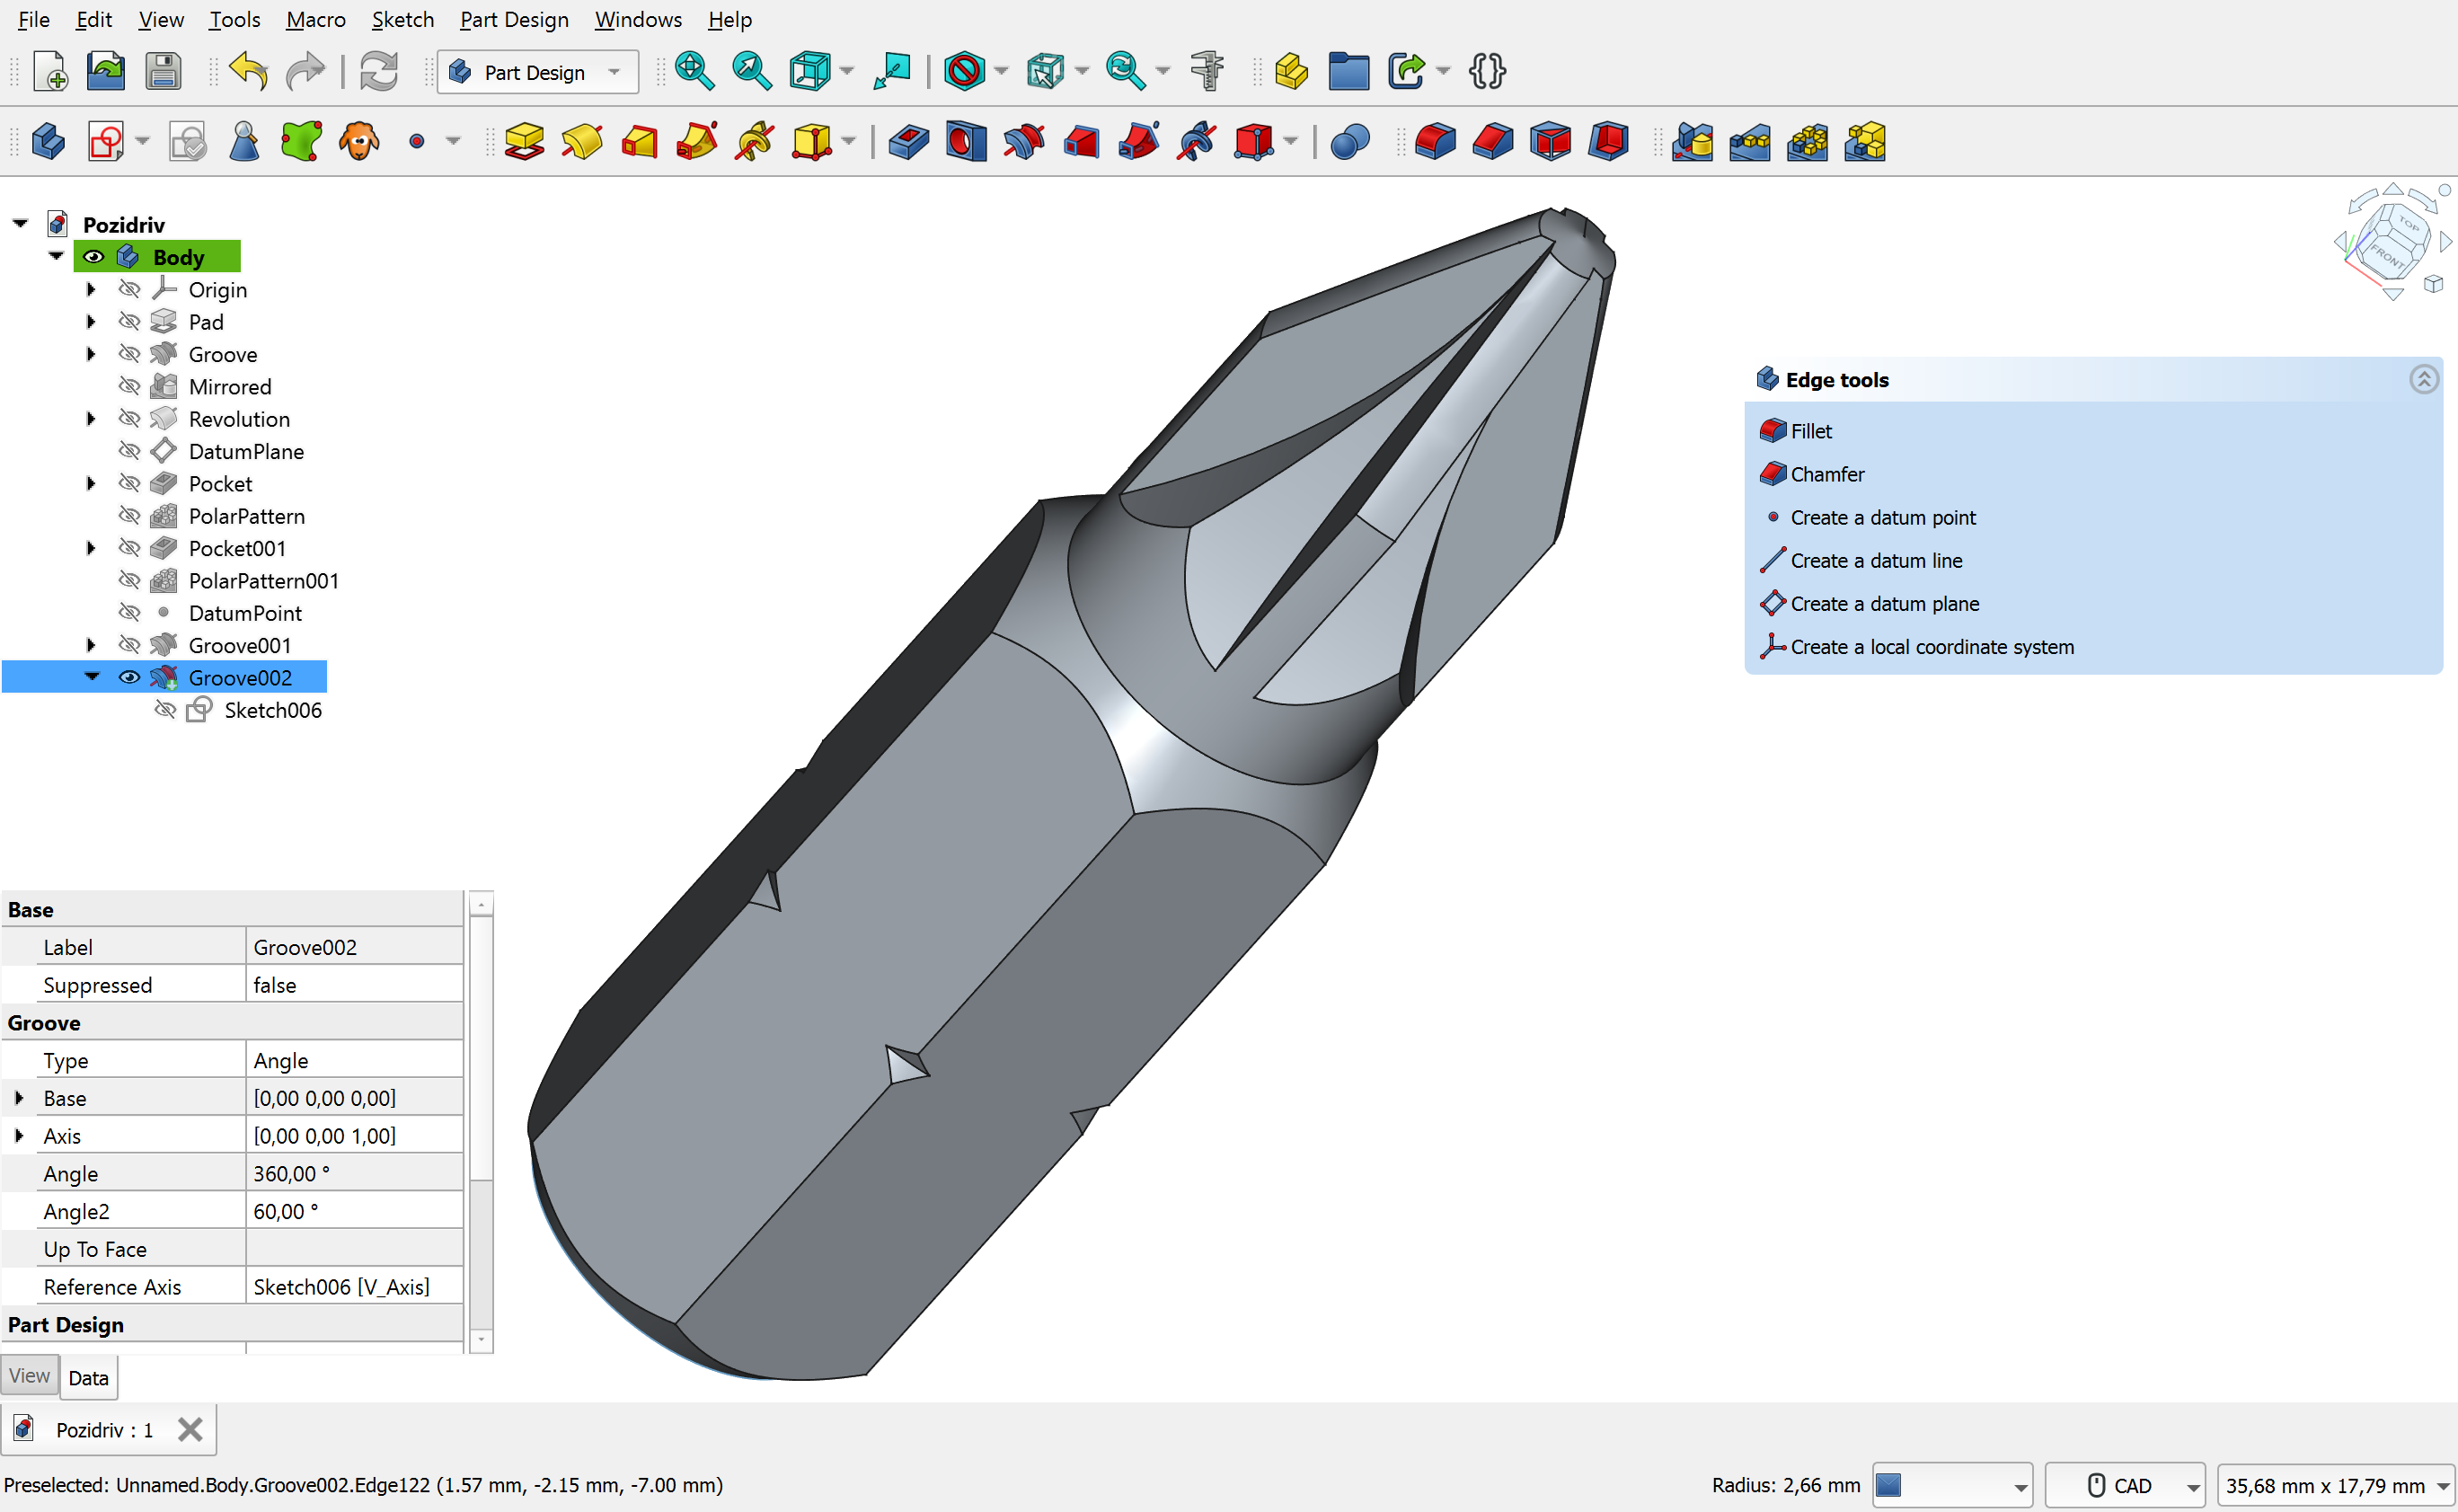
\includegraphics[width=0.8\textwidth]{img/cap1_freecad.png}
	\caption{Interfaz principal de FreeCAD con el módulo Part Design activo}
\end{figure}

FreeCAD es un software de diseño asistido por computadora (CAD)
3D de código abierto y gratuito. Permite crear modelos
paramétricos para ingeniería, arquitectura y fabricación.

%% D. Búsqueda e Inserción de Activos Gráficos
%% Imagen insertada al inicio del capítulo

%% B. Actividades Teóricas
\section{Investigar y responder}
\faPencil

Investiga sobre FreeCAD y responde:
\begin{enumerate}
	\item ¿Qué significa que FreeCAD sea de código abierto?
	\item ¿Cuáles son las principales ventajas del modelado
	      paramétrico?
	\item ¿Qué formatos de archivo puede importar y exportar
	      FreeCAD?
	\item ¿Qué lenguaje de programación se utiliza para
	      extender FreeCAD?
	\item ¿Por qué es importante usar software libre en la
	      educación técnica?
	\item Nombra tres industrias donde se utiliza FreeCAD
	      actualmente.
	\item ¿Qué diferencia a FreeCAD de otros programas CAD
	      comerciales?
	\item ¿Cuál es la licencia bajo la cual se distribuye
	      FreeCAD?
\end{enumerate}

%% C. Actividades Prácticas
\section{Resolver los siguientes problemas}
\faWrench

Problemas para aplicar conocimientos:
\begin{enumerate}
	\item Instala FreeCAD en tu computadora y verifica que
	      funcione correctamente.
	\item Localiza en la interfaz las barras de herramientas
	      principales.
	\item Abre y cierra tres archivos de ejemplo que trae
	      FreeCAD.
	\item Exporta un archivo a formato STL.
	\item Cambia el idioma de la interfaz a español.
	\item Configura el tema de color oscuro en las preferencias.
	\item Busca documentación oficial de FreeCAD en español.
	\item Identifica los workbenches disponibles en tu versión.
	\item Realiza una captura de pantalla de la interfaz y
	      anota los elementos principales.
	\item Comparte con un compañero las características
	      principales de FreeCAD.
\end{enumerate}
\chapter{Interfaz y Navegación Básica}

\begin{figure}[H]
	\centering
	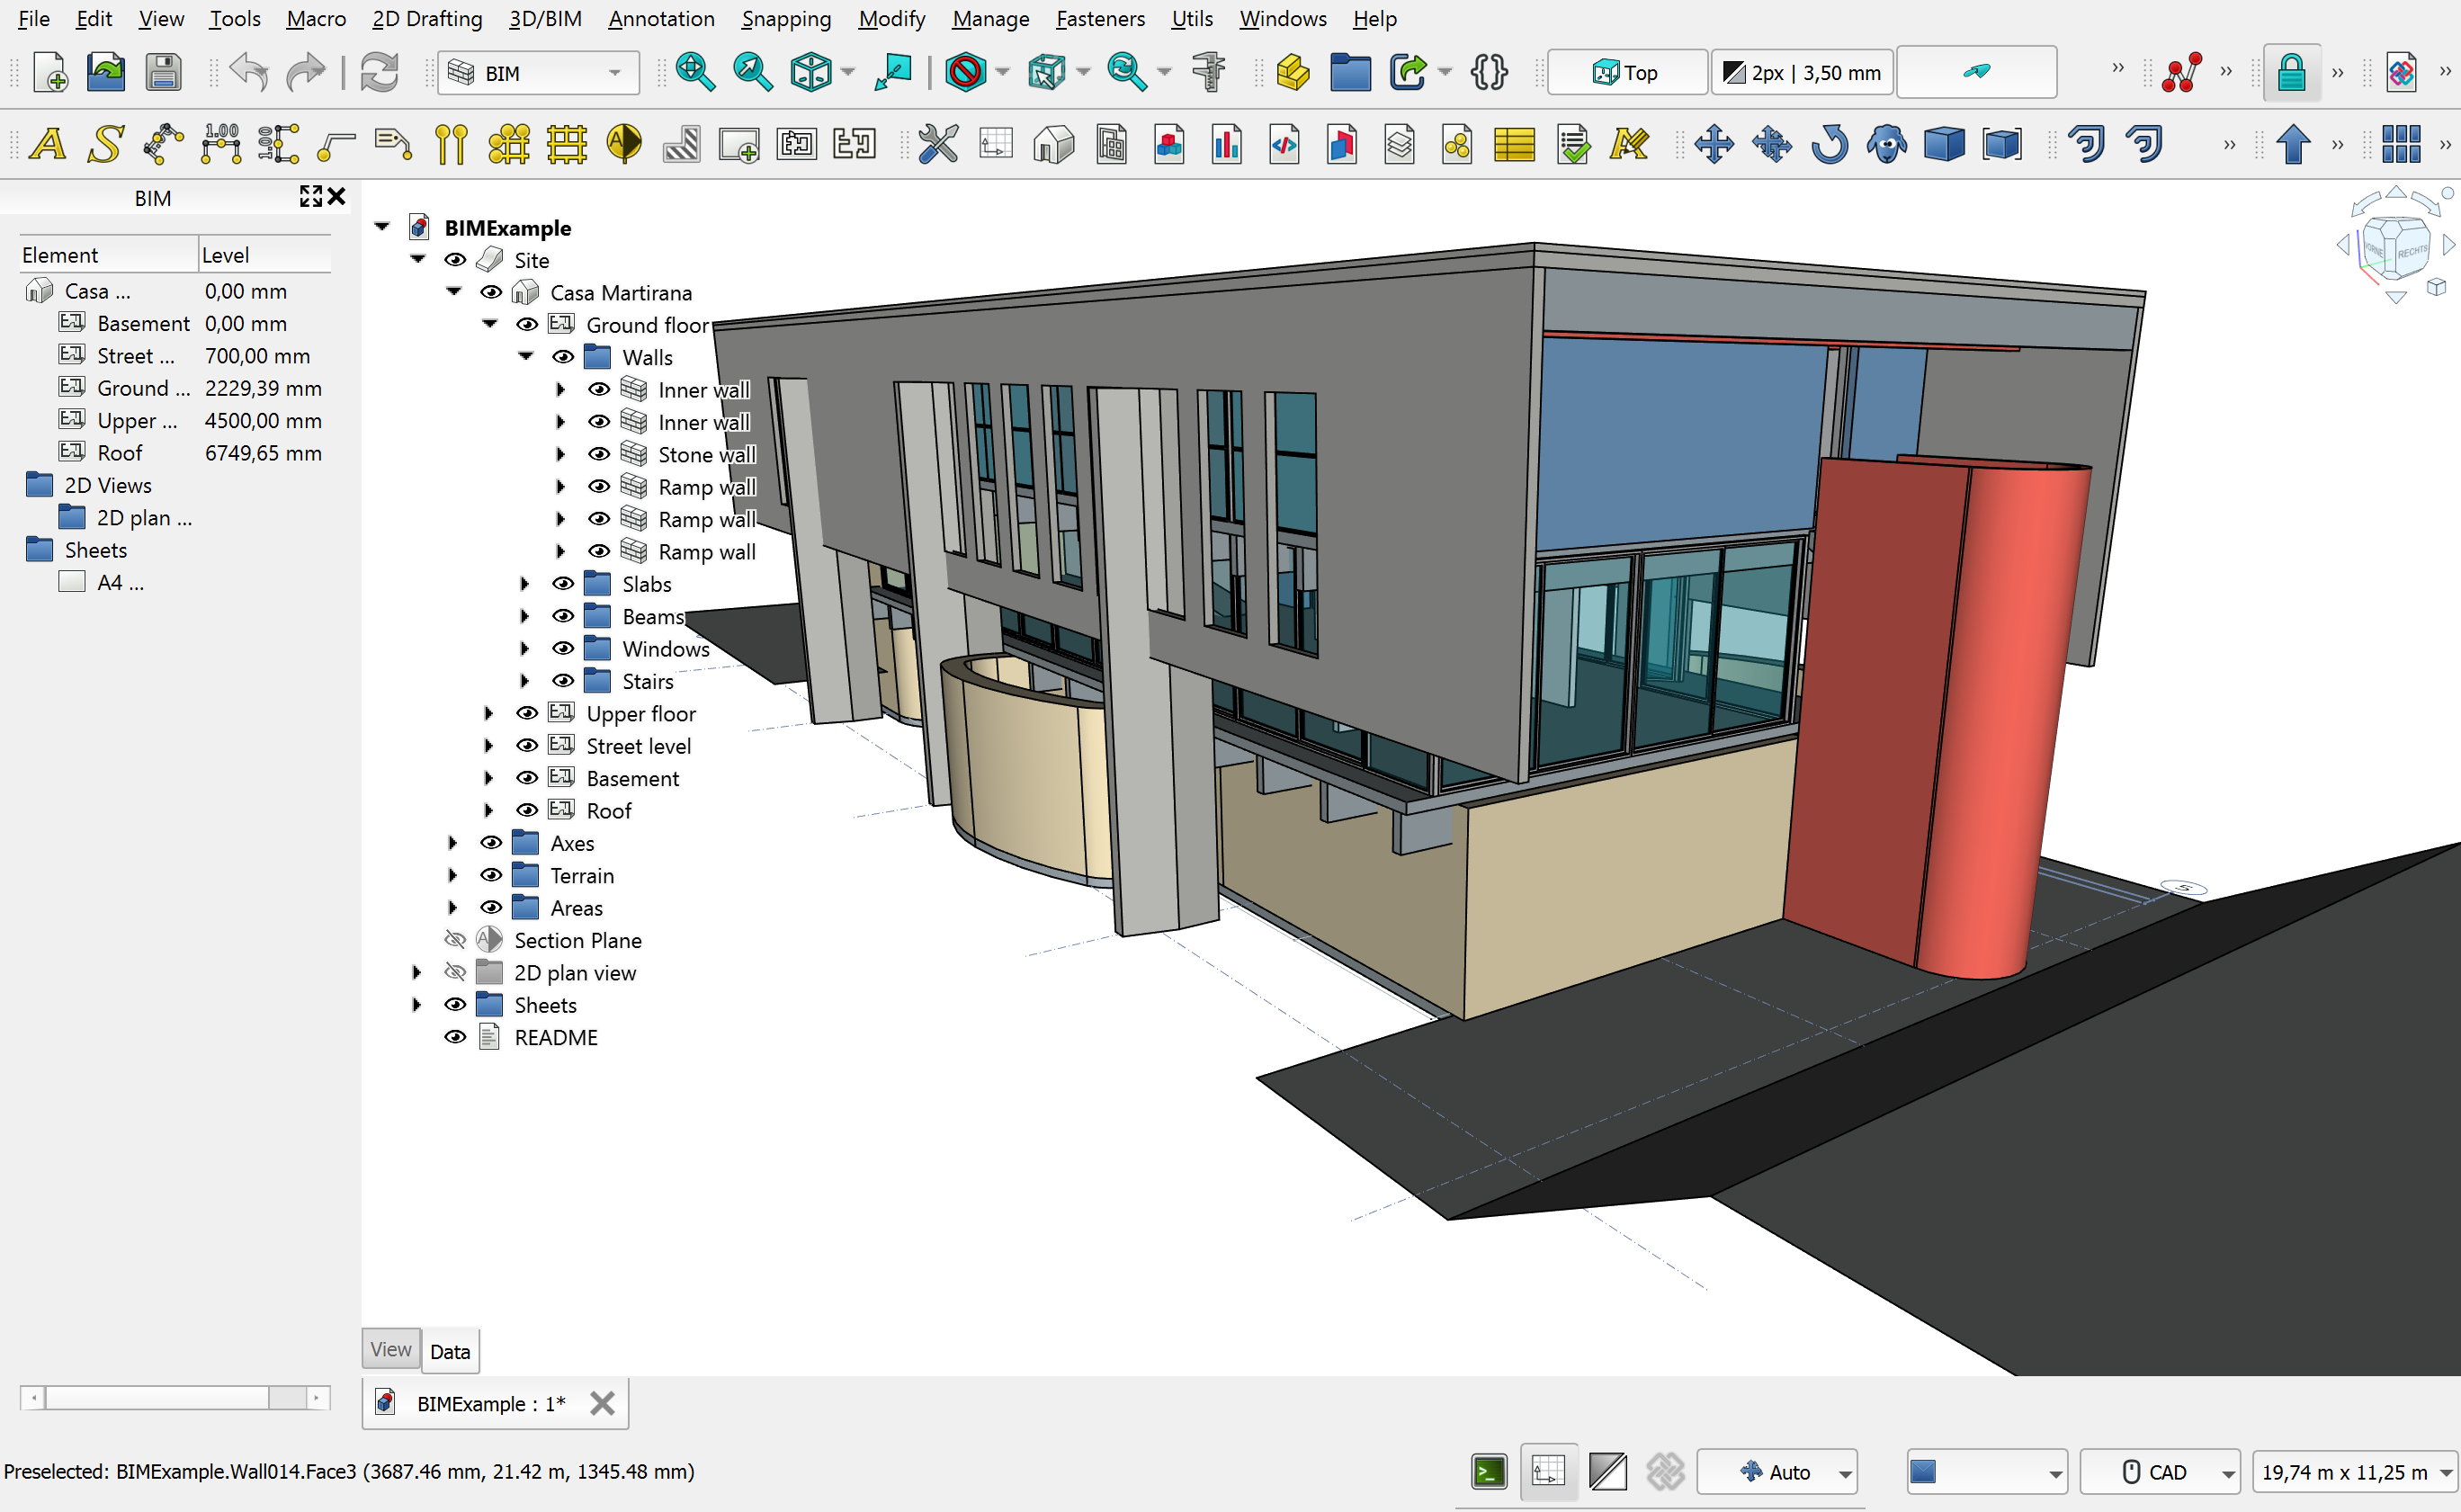
\includegraphics[width=0.8\textwidth]{img/cap2_interfaz.png}
	\caption{Vista de la interfaz de FreeCAD con área de trabajo}
\end{figure}

Aprende a moverte por FreeCAD. Conoce las áreas
principales de la interfaz y cómo navegar en 3D.

%% D. Búsqueda e Inserción de Activos Gráficos
%% Imagen insertada al inicio del capítulo

%% B. Actividades Teóricas
\section{Investigar y responder}
\faPencil

Investiga sobre la interfaz de FreeCAD y responde:
\begin{enumerate}
	\item ¿Cuáles son las áreas principales de la interfaz?
	\item ¿Qué función cumplen los workbenches o bancos de
	      trabajo?
	\item ¿Cómo se alternan entre vistas ortográficas y
	      perspectiva?
	\item ¿Qué atajos de teclado se usan para zoom, rotación
	      y desplazamiento?
	\item ¿Cómo personalizar la interfaz según tus necesidades?
	\item ¿Qué información muestra el árbol deCombo View?
	\item ¿Para qué sirve la barra de estado inferior?
	\item ¿Cómo cambiar entre diferentes workbenches?
\end{enumerate}

%% C. Actividades Prácticas
\section{Resolver los siguientes problemas}
\faWrench

Problemas para aplicar conocimientos:
\begin{enumerate}
	\item Abre FreeCAD y navega entre los diferentes
	      workbenches disponibles.
	\item Practica el zoom con la rueda del ratón y los
	      atajos de teclado.
	\item Realiza una rotación completa del espacio 3D
	      usando diferentes métodos.
	\item Cambia entre vista isométrica, frontal, lateral
	      y superior.
	\item Personaliza el tamaño y posición de los paneles
	      laterales.
	\item Guarda una configuración personalizada de
	      interfaz.
	\item Abre el archivo de ejemplo ``shaft.FCStd'' y
	      explora sus componentes en el árbol.
	\item Activa y desactiva la cuadrícula en el área de
	      trabajo.
	\item Configura las preferencias de visualización para
	      mejorar el rendimiento.
	\item Realiza una captura de pantalla con tu interfaz
	      personalizada y anota los cambios realizados.
\end{enumerate}
\chapter{Herramientas de Dibujo 2D}

\begin{figure}[H]
	\centering
	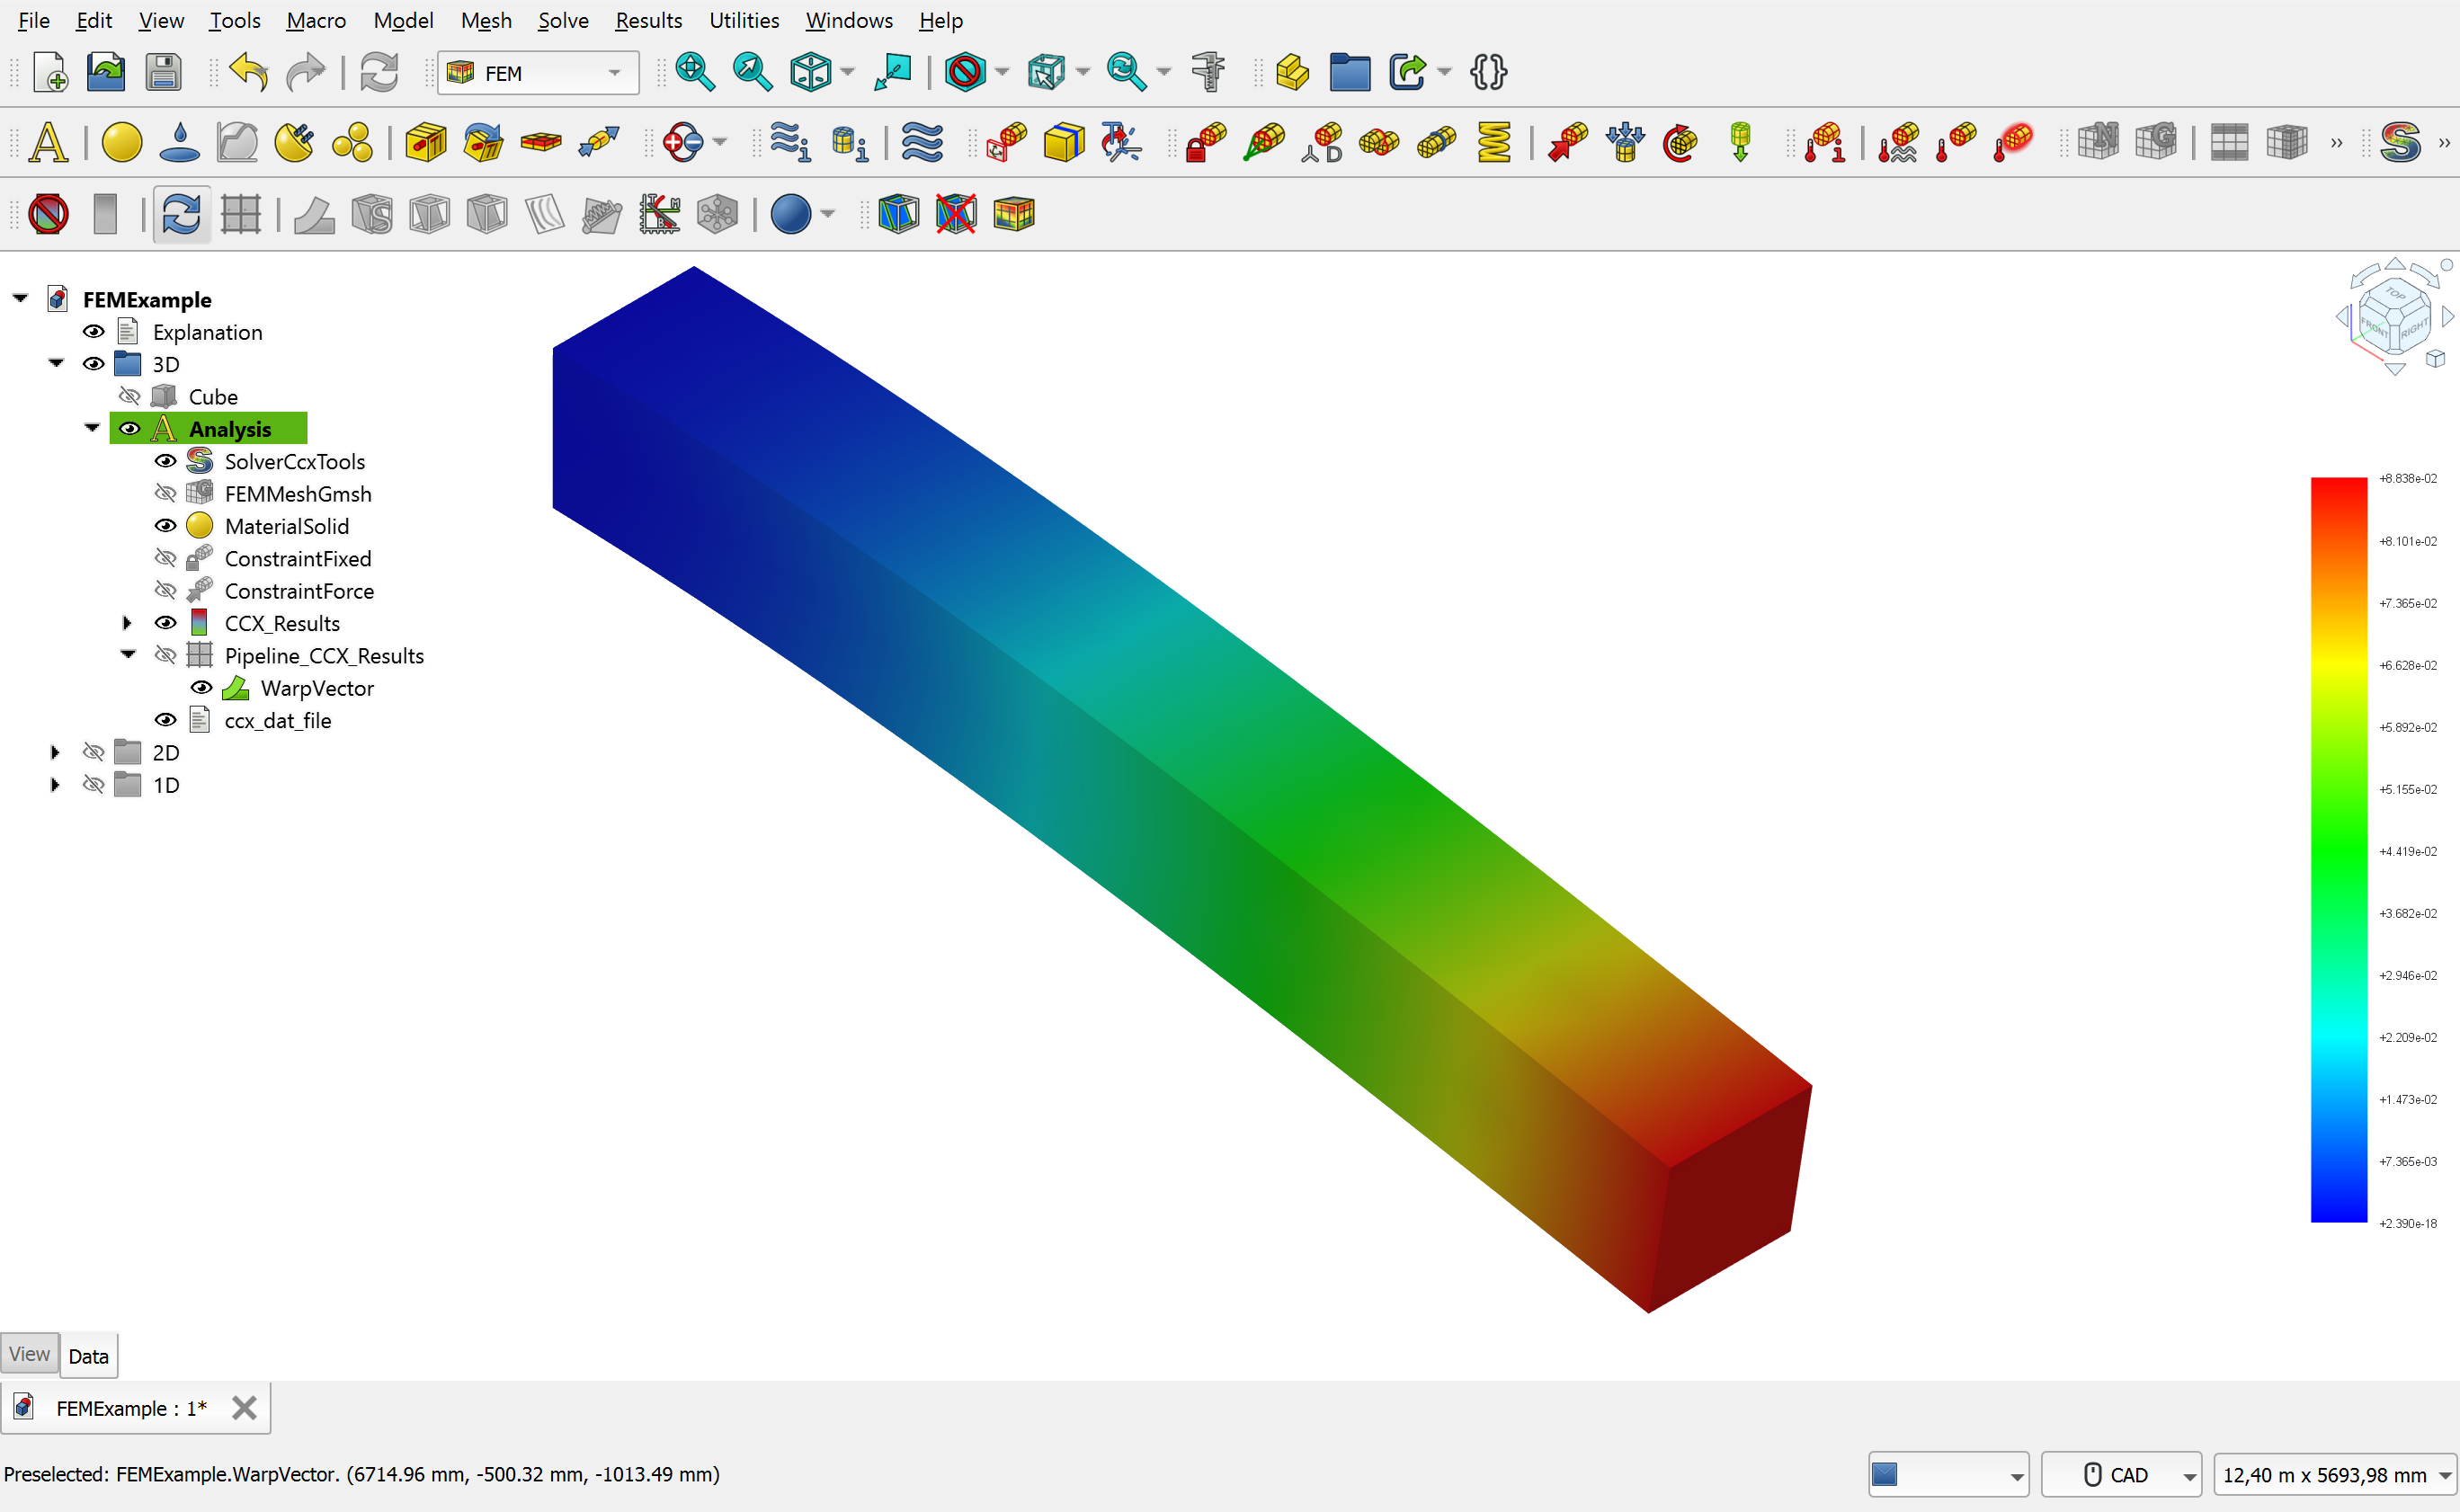
\includegraphics[width=0.8\textwidth]{img/cap3_dibujo2d.png}
	\caption{Área de dibujo 2D con elementos geométricos en FreeCAD}
\end{figure}

Aprende a usar las herramientas de dibujo 2D en FreeCAD.
Crea formas básicas y complejas usando el módulo Sketcher.

%% D. Búsqueda e Inserción de Activos Gráficos
%% Imagen insertada al inicio del capítulo

%% B. Actividades Teóricas
\section{Investigar y responder}
\faPencil

Investiga sobre dibujo 2D en FreeCAD y responde:
\begin{enumerate}
	\item ¿Qué es un boceto o sketch en FreeCAD?
	\item ¿Cuáles son las herramientas básicas de dibujo 2D?
	\item ¿Qué diferencia hay entre líneas, círculos y arcos?
	\item ¿Cómo se crean polígonos regulares e irregulares?
	\item ¿Qué son las polilíneas y cuándo se utilizan?
	\item ¿Cómo importar geometría 2D desde archivos DXF?
	\item ¿Qué herramientas sirven para modificar formas 2D?
	\item ¿Cómo trabajar con capas en dibujo 2D?
\end{enumerate}

%% C. Actividades Prácticas
\section{Resolver los siguientes problemas}
\faWrench

Problemas para aplicar conocimientos:
\begin{enumerate}
	\item Crea un nuevo archivo y activa el módulo Sketcher.
	\item Dibuja un rectángulo de 100x50 mm con
	      dimensiones exactas.
	\item Crea un círculo de radio 25 mm en el centro del
	      plano.
	\item Dibuja un triángulo equilátero de lado 40 mm.
	\item Crea una figura combinando rectángulos y círculos
	      para formar una llave inglesa simple.
	\item Practica el uso de la herramienta de arco con
	      diferentes ángulos.
	\item Dibuja una estrella de cinco puntas usando
	      polilíneas.
	\item Importa un archivo DXF y modifica su geometría.
	\item Crea un plano simple de una pieza mecánica básica.
	\item Organiza tus dibujos en diferentes capas y
	      asigna colores.
\end{enumerate}
\chapter{Modelado 3D Básico}

\begin{figure}[H]
	\centering
	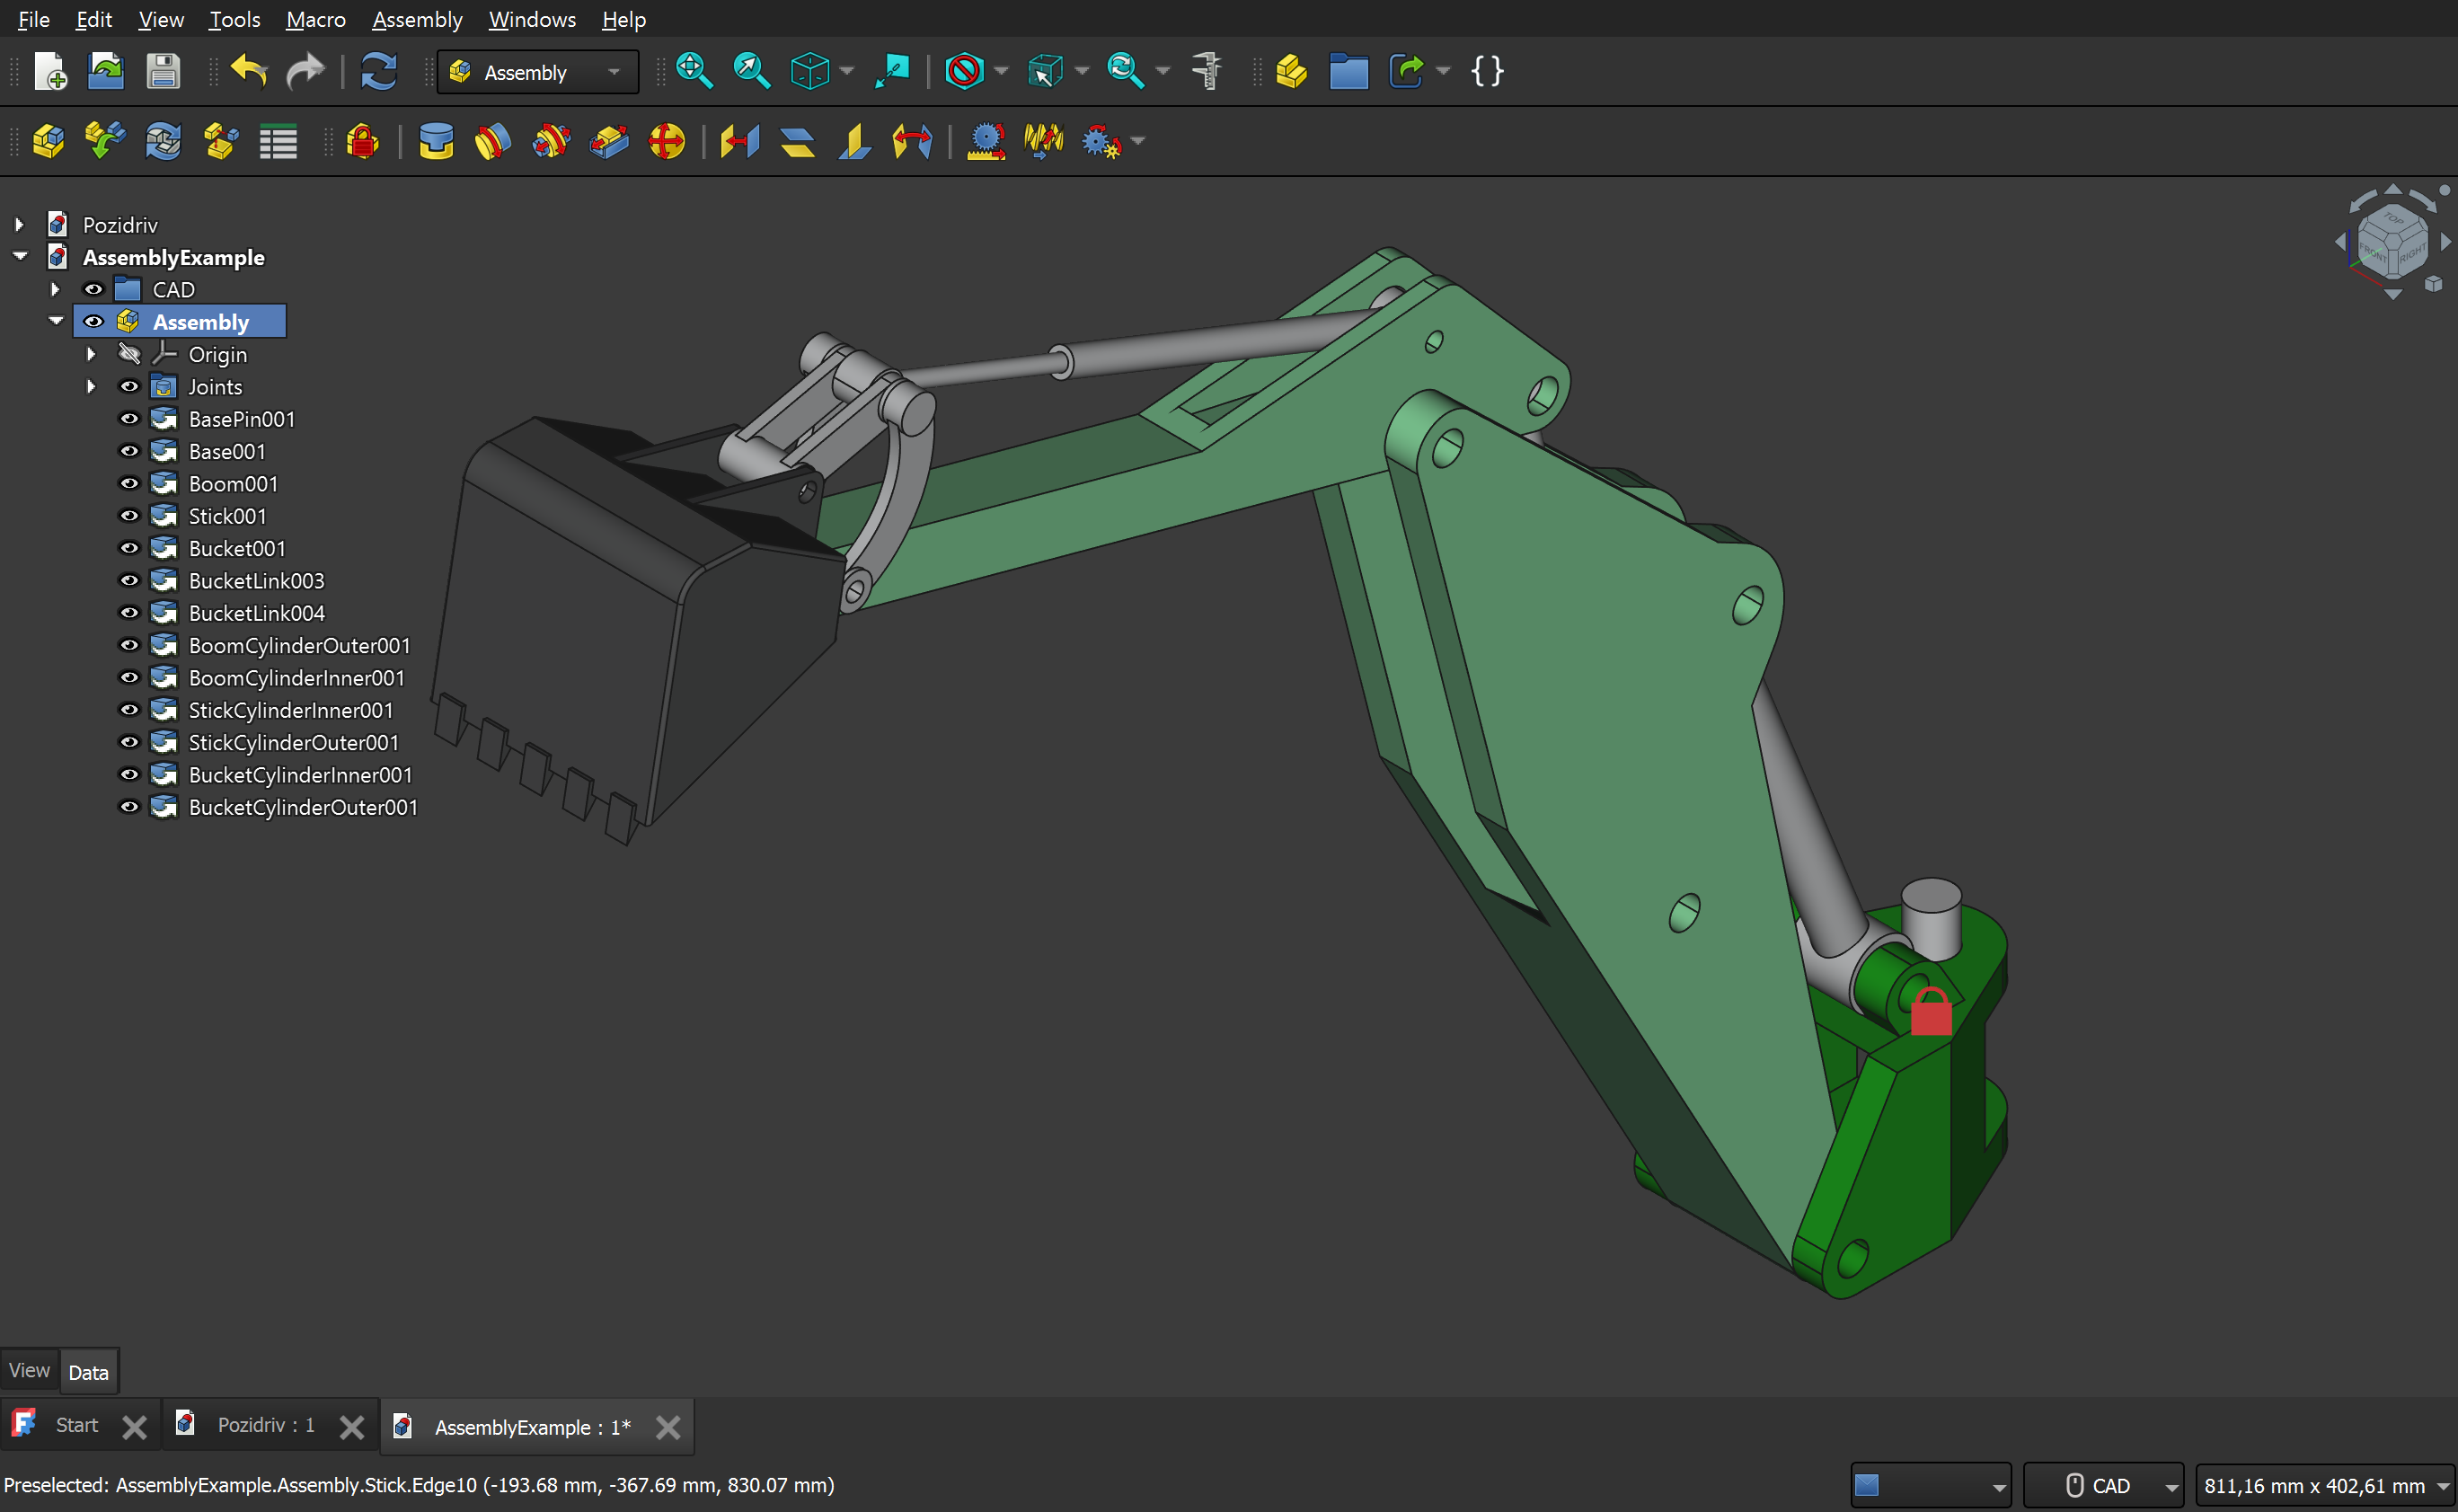
\includegraphics[width=0.8\textwidth]{img/cap4_modelado3d.png}
	\caption{Modelo 3D de ensamblaje creado en FreeCAD}
\end{figure}

Aprende los fundamentos del modelado 3D en FreeCAD.
Crea sólidos simples y entiende el concepto de
modelado paramétrico.

%% D. Búsqueda e Inserción de Activos Gráficos
%% Imagen insertada al inicio del capítulo

%% B. Actividades Teóricas
\section{Investigar y responder}
\faPencil

Investiga sobre modelado 3D en FreeCAD y responde:
\begin{enumerate}
	\item ¿Qué es el modelado sólido (solid modeling)?
	\item ¿Cuáles son las formas geométricas básicas en 3D?
	\item ¿Cómo se relacionan los bocetos 2D con los
	      sólidos 3D?
	\item ¿Qué es una operación booleana en modelado 3D?
	\item ¿Cómo se unen y separan sólidos en FreeCAD?
	\item ¿Qué significa que el modelado sea paramétrico?
	\item ¿Cómo se modifican las dimensiones después de
	      crear un sólido?
	\item ¿Qué son las características (features) en
	      FreeCAD?
\end{enumerate}

%% C. Actividades Prácticas
\section{Resolver los siguientes problemas}
\faWrench

Problemas para aplicar conocimientos:
\begin{enumerate}
	\item Crea un cubo de 50x50x50 mm usando la herramienta
	      de caja.
	\item Modela un cilindro de radio 20 mm y altura 40 mm.
	\item Crea una esfera de radio 25 mm.
	\item Modela una pieza combinando cubo y cilindro con
	      operación de unión.
	\item Crea un agujero cilíndrico en un cubo usando
	      operación de sustracción.
	\item Modela un prisma hexagonal de lado 15 mm y altura
	      30 mm.
	\item Crea una pieza con varios sólidos y guárdala como
	      archivo FreeCAD.
	\item Practica la modificación de dimensiones en un
	      modelo existente.
	\item Modela una pieza simple que simule una tuercas
	      mecánica.
	\item Exporta tu modelo a formato STEP para usar en
	      otros programas.
\end{enumerate}
\chapter{Restricciones y Cotas}

\begin{figure}[H]
	\centering
	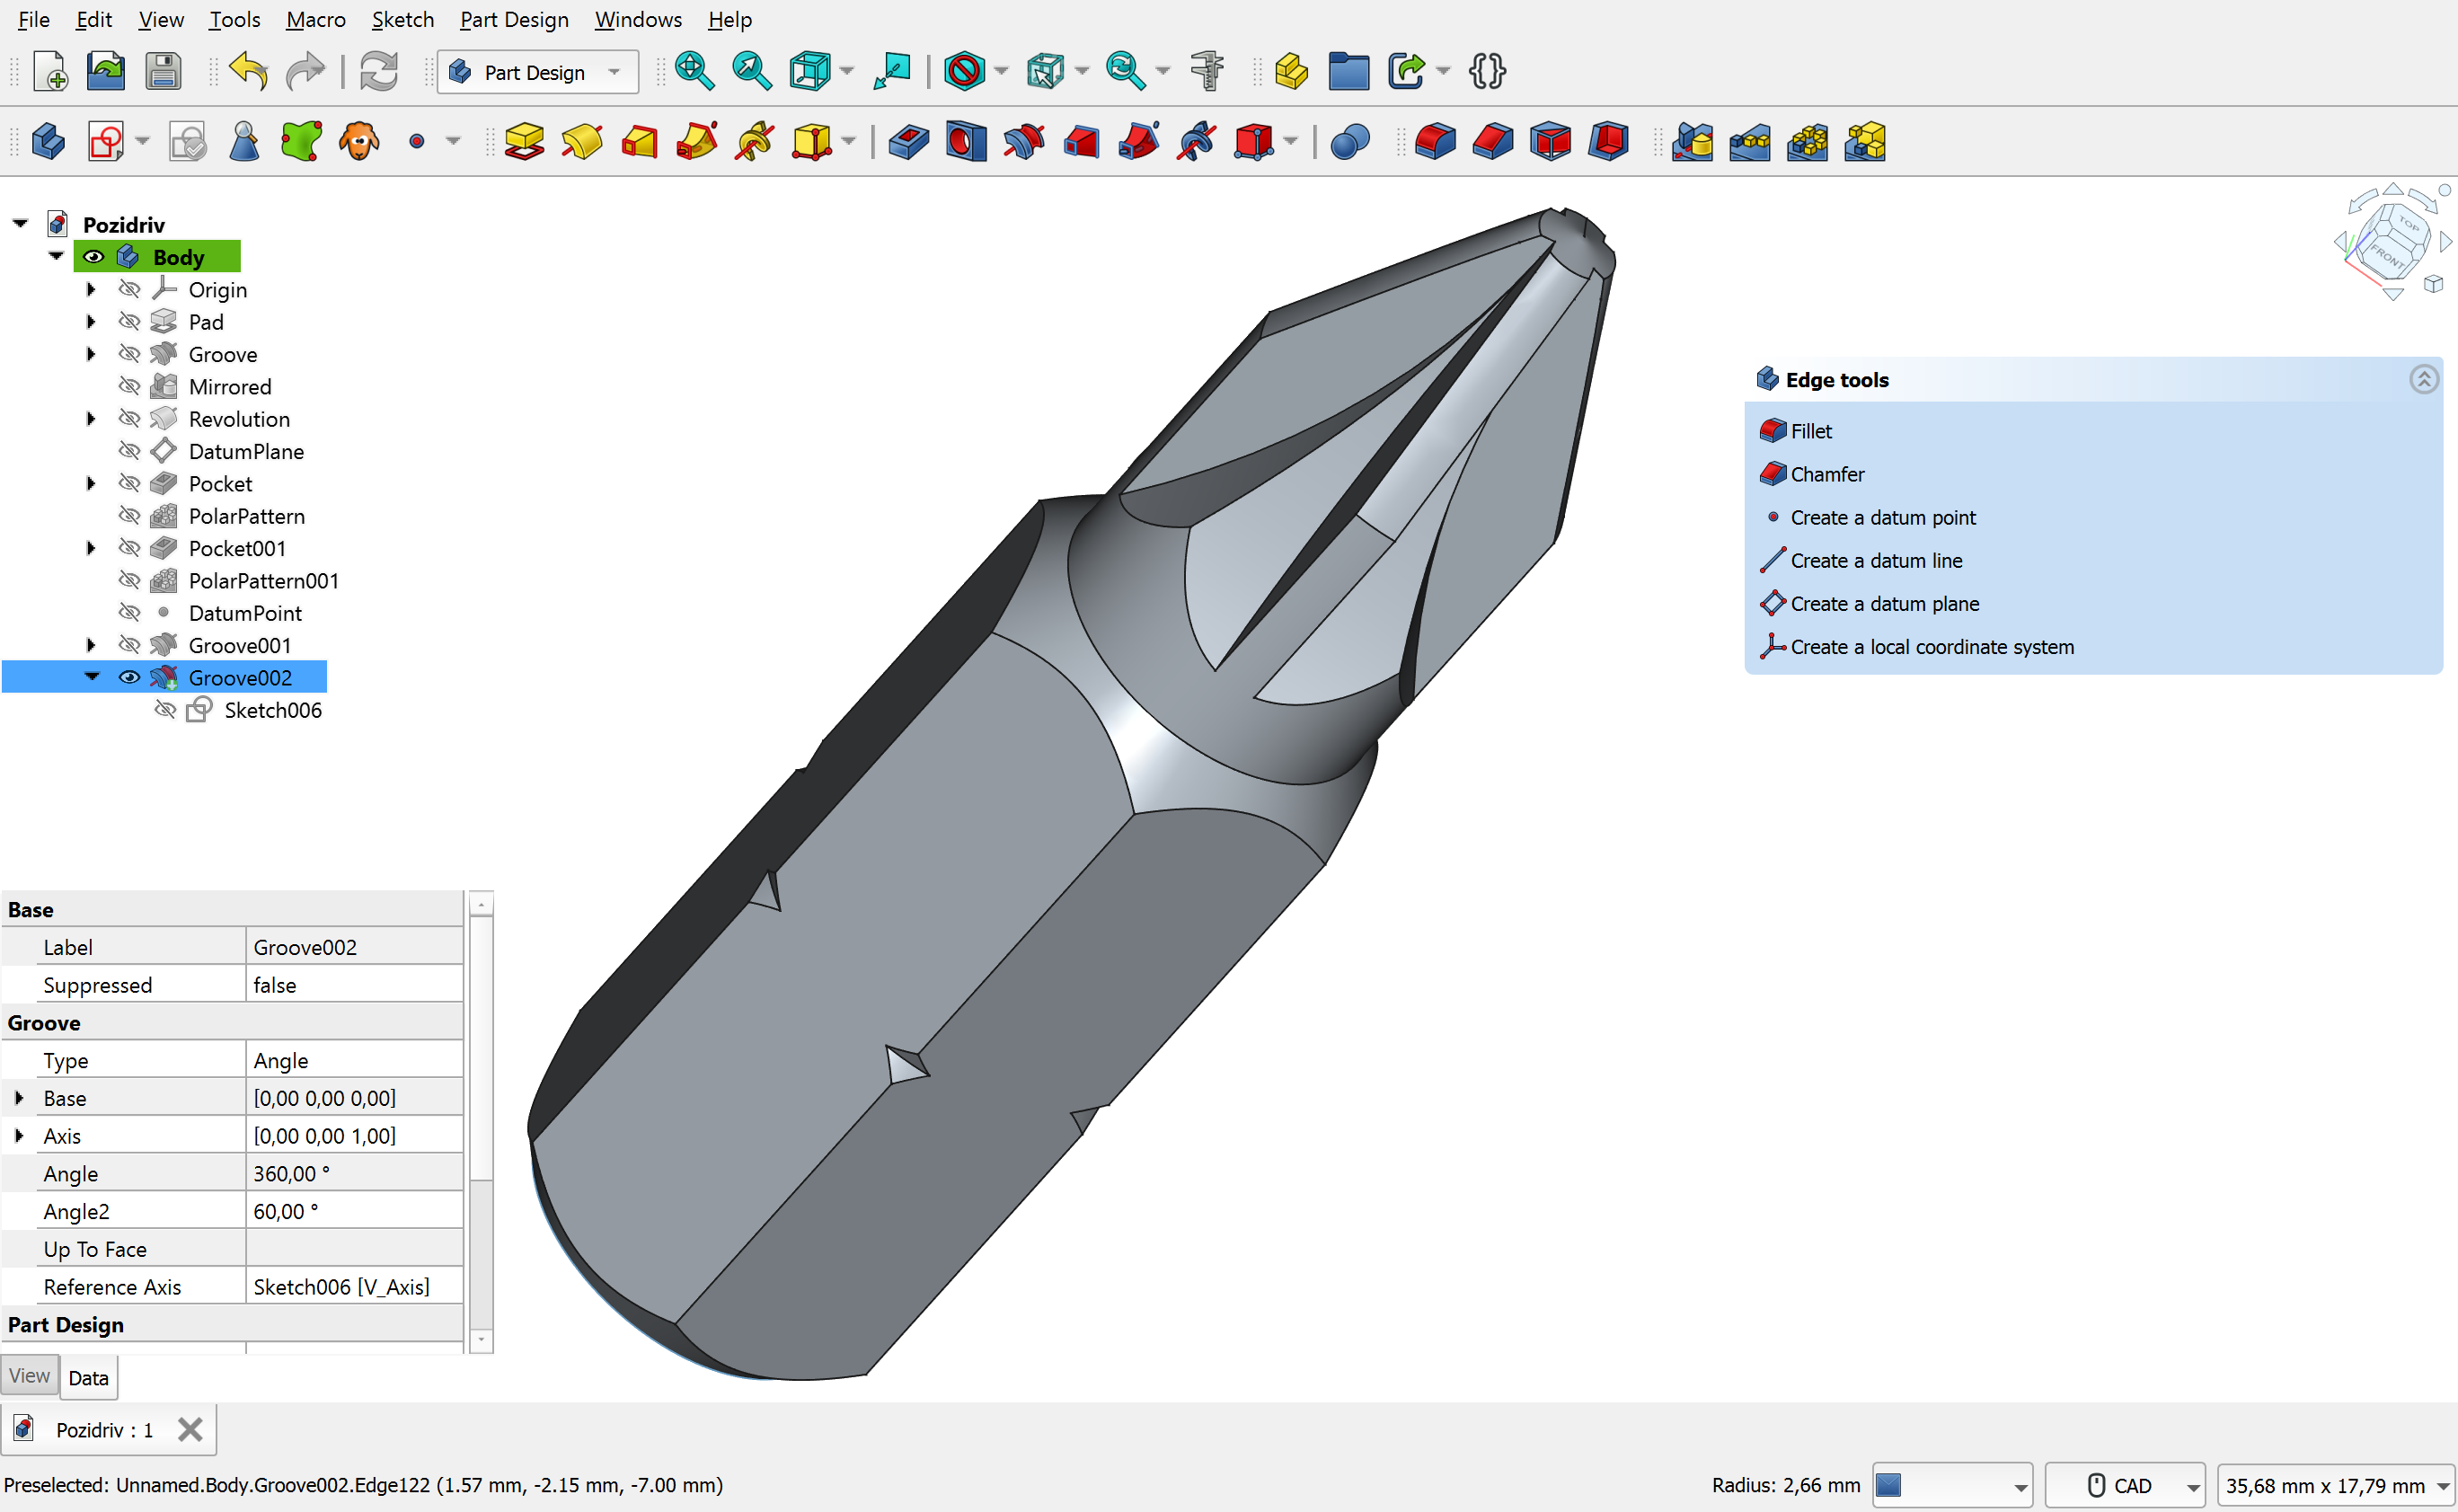
\includegraphics[width=0.8\textwidth]{img/cap5_restricciones.png}
	\caption{Boceto con restricciones geométricas y dimensionales}
\end{figure}

Aprende a aplicar restricciones geométricas y cotas
dimensionales a tus bocetos. El control preciso de
dimensiones es fundamental en diseño paramétrico.

%% D. Búsqueda e Inserción de Activos Gráficos
%% Imagen insertada al inicio del capítulo

%% B. Actividades Teóricas
\section{Investigar y responder}
\faPencil

Investiga sobre restricciones en FreeCAD y responde:
\begin{enumerate}
	\item ¿Qué son las restricciones geométricas en un
	      boceto?
	\item ¿Cuál es la diferencia entre restricciones
	      geométricas y dimensionales?
	\item ¿Qué restricciones se aplican a líneas paralelas
	      y perpendiculares?
	\item ¿Cómo se fijan longitudes y ángulos exactos?
	\item ¿Qué es una cota y cómo se edita?
	\item ¿Qué significa ``fully constrained'' en un boceto?
	\item ¿Cómo se aplican restricciones de simetría?
	\item ¿Qué errores comunes ocurren al aplicar
	      restricciones?
\end{enumerate}

%% C. Actividades Prácticas
\section{Resolver los siguientes problemas}
\faWrench

Problemas para aplicar conocimientos:
\begin{enumerate}
	\item Crea un rectángulo con restricciones de igual
	      longitud en los lados opuestos.
	\item Dibuja dos líneas paralelas y aplica restricción
	      de distancia entre ellas.
	\item Crea un triángulo con restricciones de igual
	      longitud en los tres lados.
	\item Dibuja un círculo inscrito en un cuadrado usando
	      restricciones de tangencia.
	\item Crea una figura con restricciones de perpendicularidad
	      entre líneas.
	\item Aplica restricciones de simetría a una figura
	      respecto a un eje.
	\item Modifica las cotas de un boceto existente y
	      observa cómo cambia la forma.
	\item Crea un boceto completamente restringido de una
	      pieza mecánica simple.
	\item Identifica y corrige restricciones conflictivas
	      en un boceto.
	\item Practica la edición masiva de cotas en un boceto
	      complejo.
\end{enumerate}
\chapter{Operaciones de Modelado}

\begin{figure}[H]
	\centering
	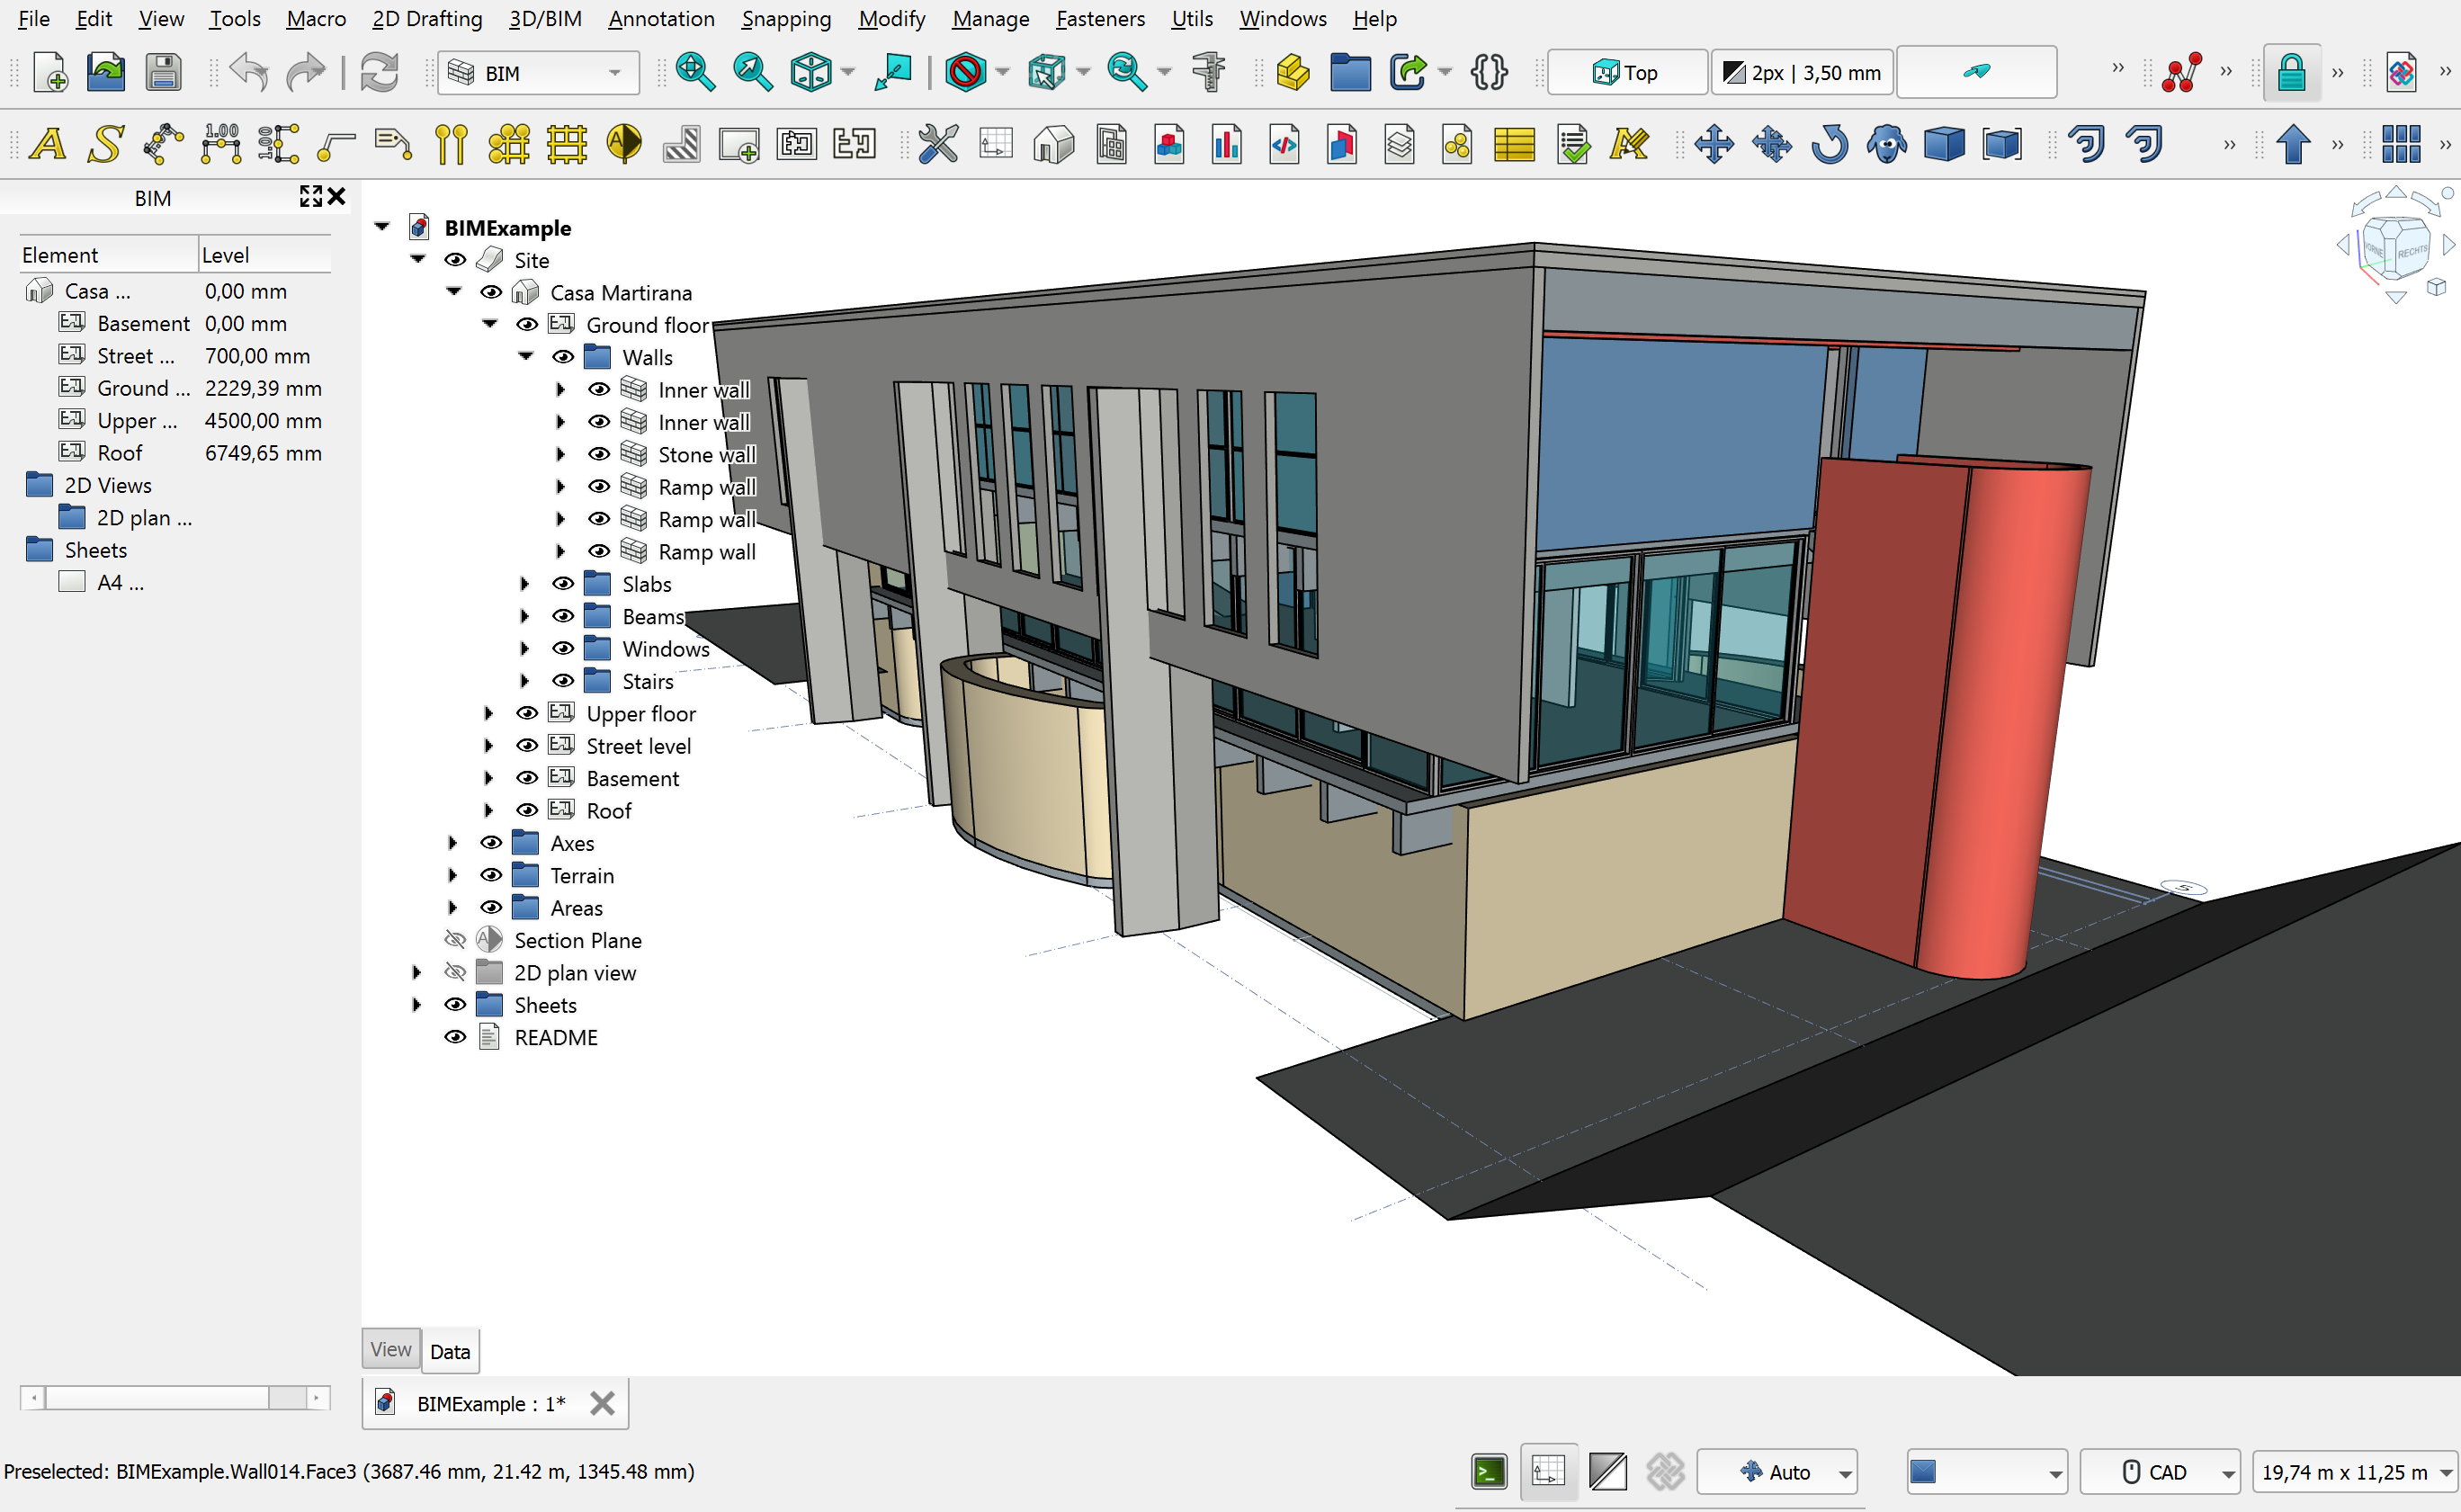
\includegraphics[width=0.8\textwidth]{img/cap6_operaciones.png}
	\caption{Modelo 3D creado con operaciones de extrusión y revolución}
\end{figure}

Aprende las operaciones fundamentales de modelado 3D:
extrusión, revolución y loft. Convierte bocetos 2D
en sólidos complejos.

%% D. Búsqueda e Inserción de Activos Gráficos
%% Imagen insertada al inicio del capítulo

%% B. Actividades Teóricas
\section{Investigar y responder}
\faPencil

Investiga sobre operaciones de modelado y responde:
\begin{enumerate}
	\item ¿Qué es la operación de extrusión (pad) y cómo
	      se aplica?
	\item ¿Cómo funciona la operación de revolución (revolve)?
	\item ¿Qué es la operación de loft y cuándo se utiliza?
	\item ¿Cómo se crean agujeros (pockets) en sólidos?
	\item ¿Qué es el biselado (fillet) y el chaflanado
	      (chamfer)?
	\item ¿Cómo se combinan múltiples operaciones en un
	      modelo?
	\item ¿Qué significa ``historial de operaciones'' en
	      FreeCAD?
	\item ¿Cómo se modifican operaciones después de creadas?
\end{enumerate}

%% C. Actividades Prácticas
\section{Resolver los siguientes problemas}
\faWrench

Problemas para aplicar conocimientos:
\begin{enumerate}
	\item Crea un prisma rectangular extrusionando un
	      rectángulo de 100x50 mm a 30 mm de altura.
	\item Modela un cilindro hueco usando la operación
	      de revolución.
	\item Crea una pieza con múltiples extrusiones de
	      diferentes alturas.
	\item Modela una pieza con agujero cilíndrico pasante.
	\item Practica el biselado de aristas con diferentes
	      radios.
	\item Crea un chaflán de 45 grados en las aristas
	      de un cubo.
	\item Modela una pieza simple de una hélice usando
	      operación de loft.
	\item Crea una pieza que combine extrusión y
	      revolución.
	\item Modifica la altura de una extrusión en un modelo
	      existente.
	\item Modela una pieza mecánica simple como un soporte
	      con varias operaciones.
\end{enumerate}
\chapter{Módulos Especializados}

\begin{figure}[H]
	\centering
	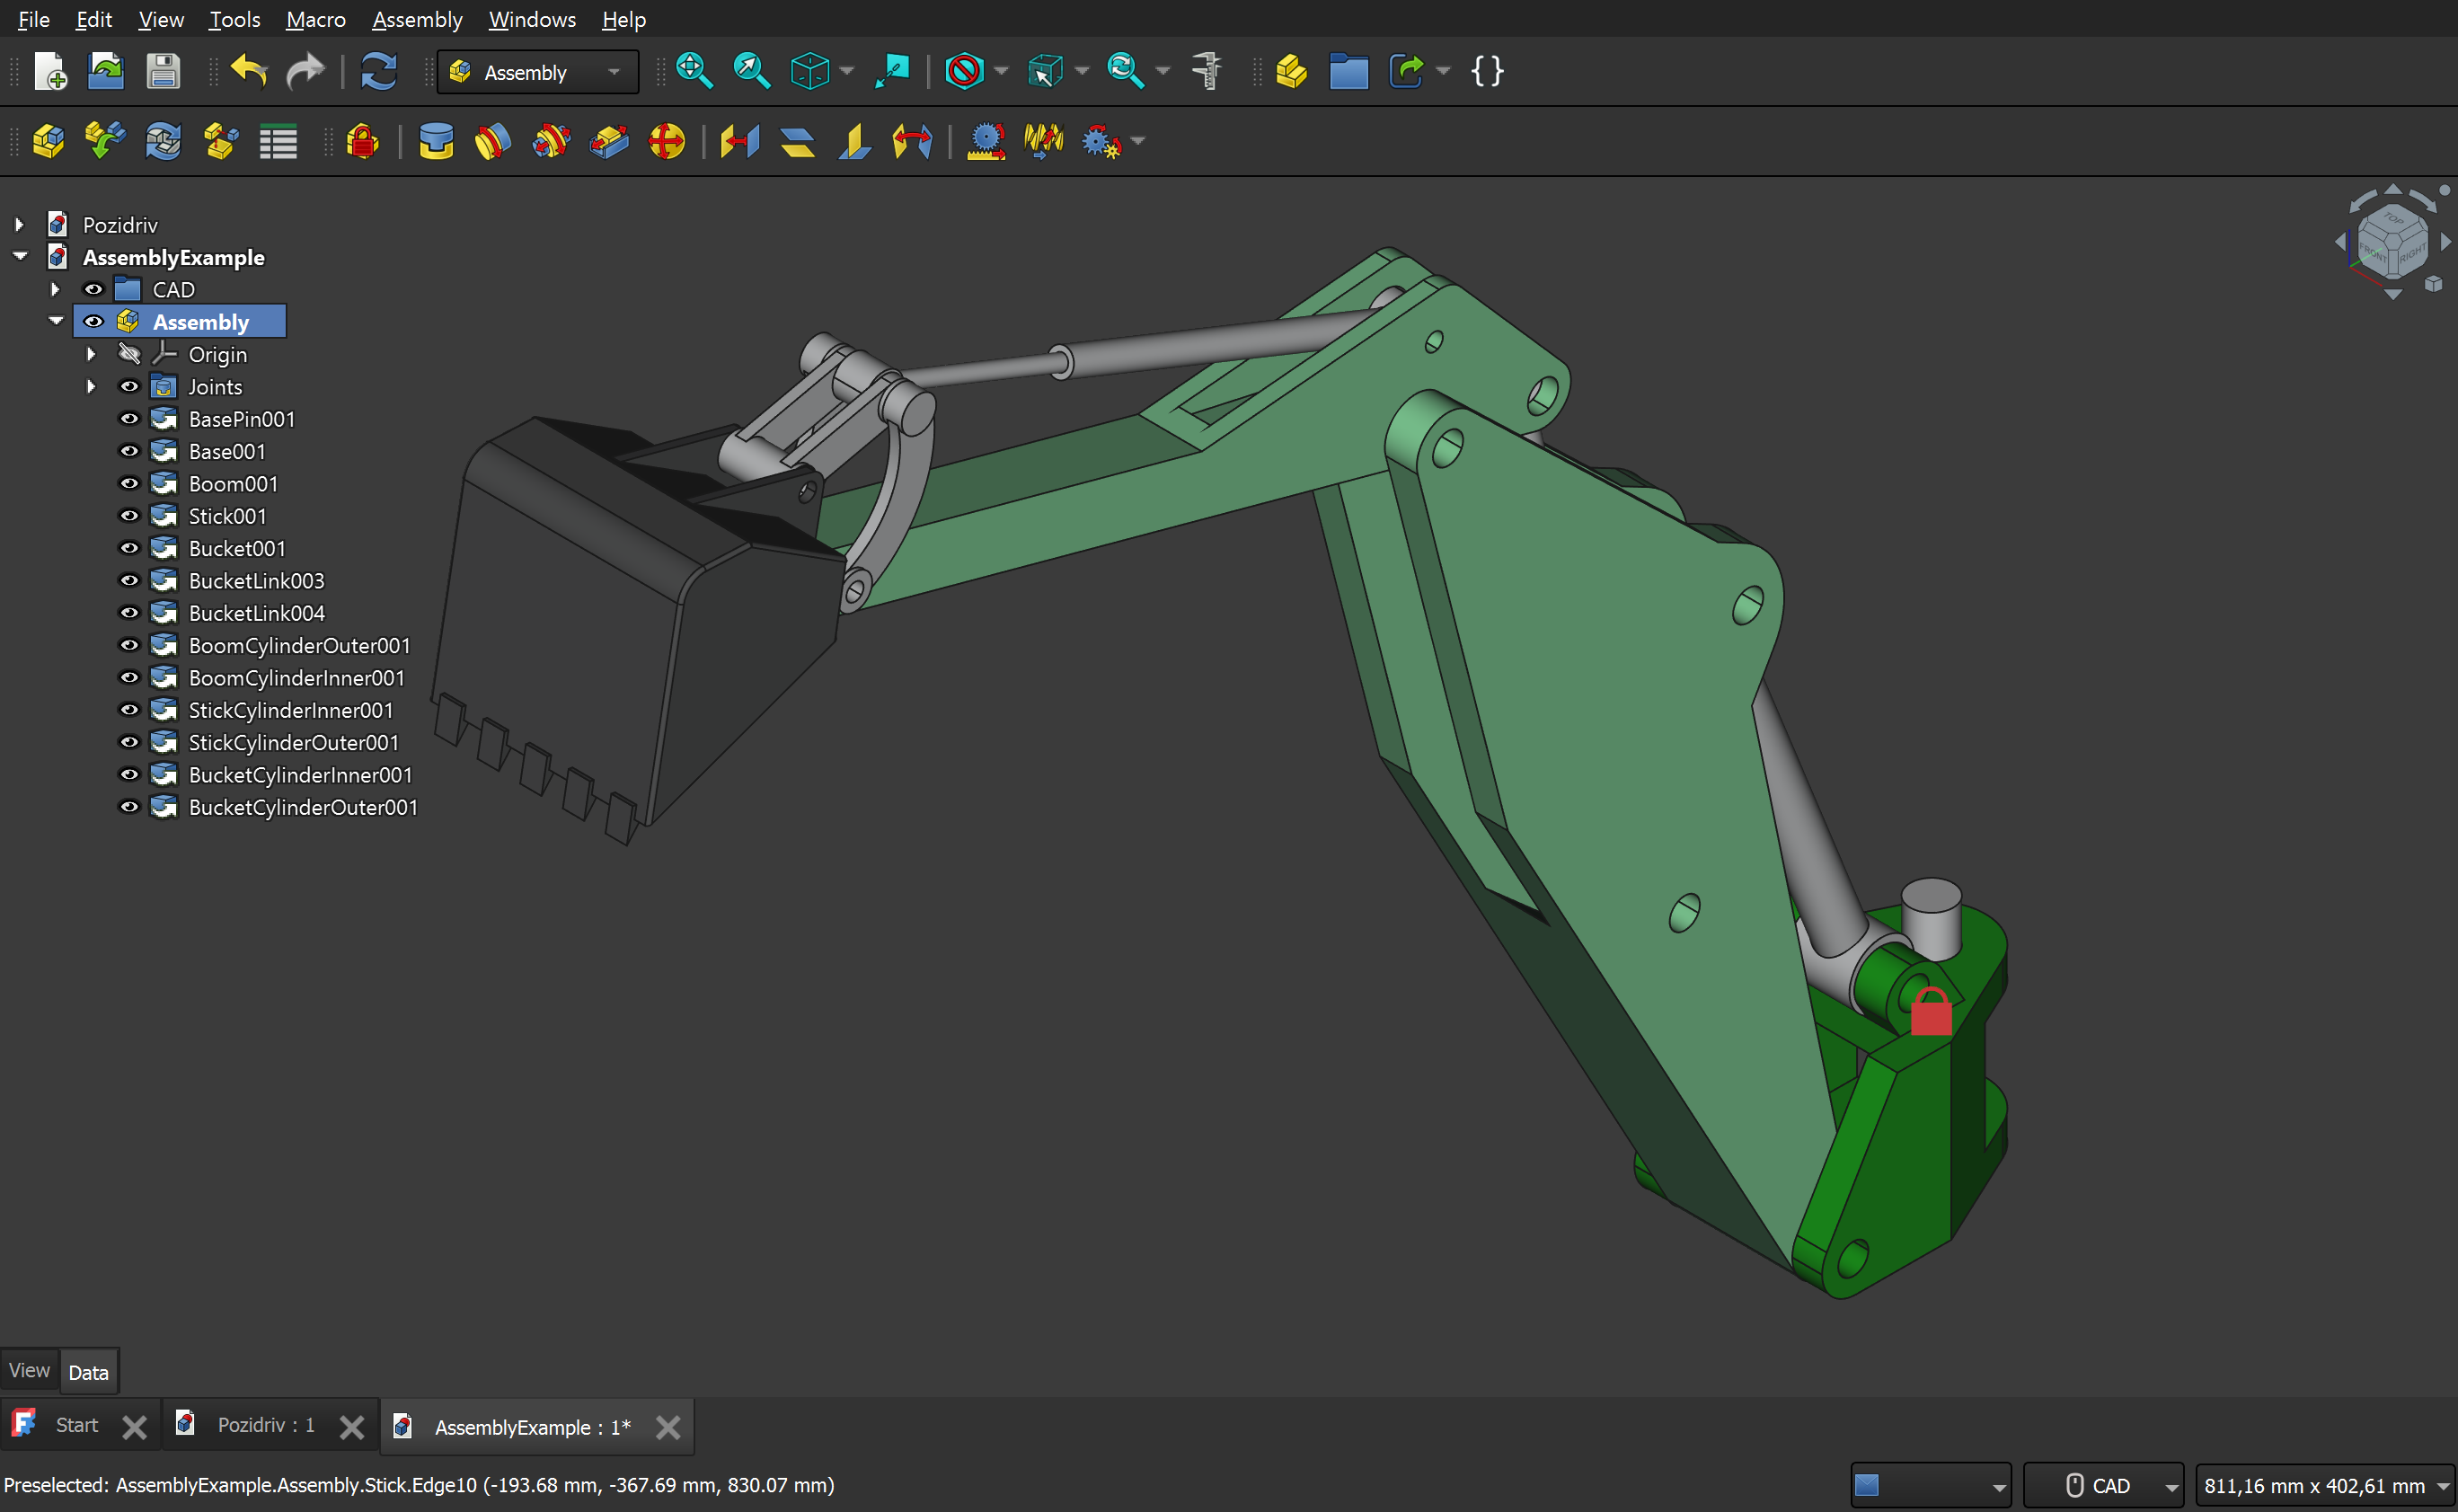
\includegraphics[width=0.8\textwidth]{img/cap7_modulos.png}
	\caption{Módulos especializados de FreeCAD en acción}
\end{figure}

Conoce los módulos especializados de FreeCAD: Part
Design, Sketcher, Draft y otros. Cada módulo está
diseñado para tareas específicas de diseño.

%% D. Búsqueda e Inserción de Activos Gráficos
%% Imagen insertada al inicio del capítulo

%% B. Actividades Teóricas
\section{Investigar y responder}
\faPencil

Investiga sobre módulos de FreeCAD y responde:
\begin{enumerate}
	\item ¿Cuál es la diferencia entre Part y Part Design?
	\item ¿Qué funciones específicas tiene el módulo Sketcher?
	\item ¿Para qué sirve el módulo Draft en FreeCAD?
	\item ¿Qué ventajas ofrece el módulo Arch para
	      arquitectura?
	\item ¿Cómo se cambia entre diferentes workbenches?
	\item ¿Qué módulos son esenciales para diseño mecánico?
	\item ¿Cómo se instalan módulos adicionales o plugins?
	\item ¿Qué módulos son recomendados para principiantes?
\end{enumerate}

%% C. Actividades Prácticas
\section{Resolver los siguientes problemas}
\faWrench

Problemas para aplicar conocimientos:
\begin{enumerate}
	\item Explora el módulo Part Design y crea una pieza
	      simple.
	\item Usa el módulo Sketcher para crear un boceto
	      complejo con restricciones.
	\item Trabaja con el módulo Draft para crear geometría
	      2D con proyección a 3D.
	\item Explora el módulo Arch y crea una pared simple.
	\item Compara las herramientas de Part y Part Design
	      para la misma tarea.
	\item Crea una pieza usando el flujo de trabajo de
	      Part Design.
	\item Instala un módulo adicional desde el administrador
	      de complementos.
	\item Personaliza tu barra de herramientas con accesos
	      directos a módulos.
	\item Crea un archivo que combine herramientas de
	      múltiples módulos.
	\item Documenta las diferencias entre al menos tres
	      módulos de FreeCAD.
\end{enumerate}
\chapter{Planos Técnicos}

\begin{figure}[H]
	\centering
	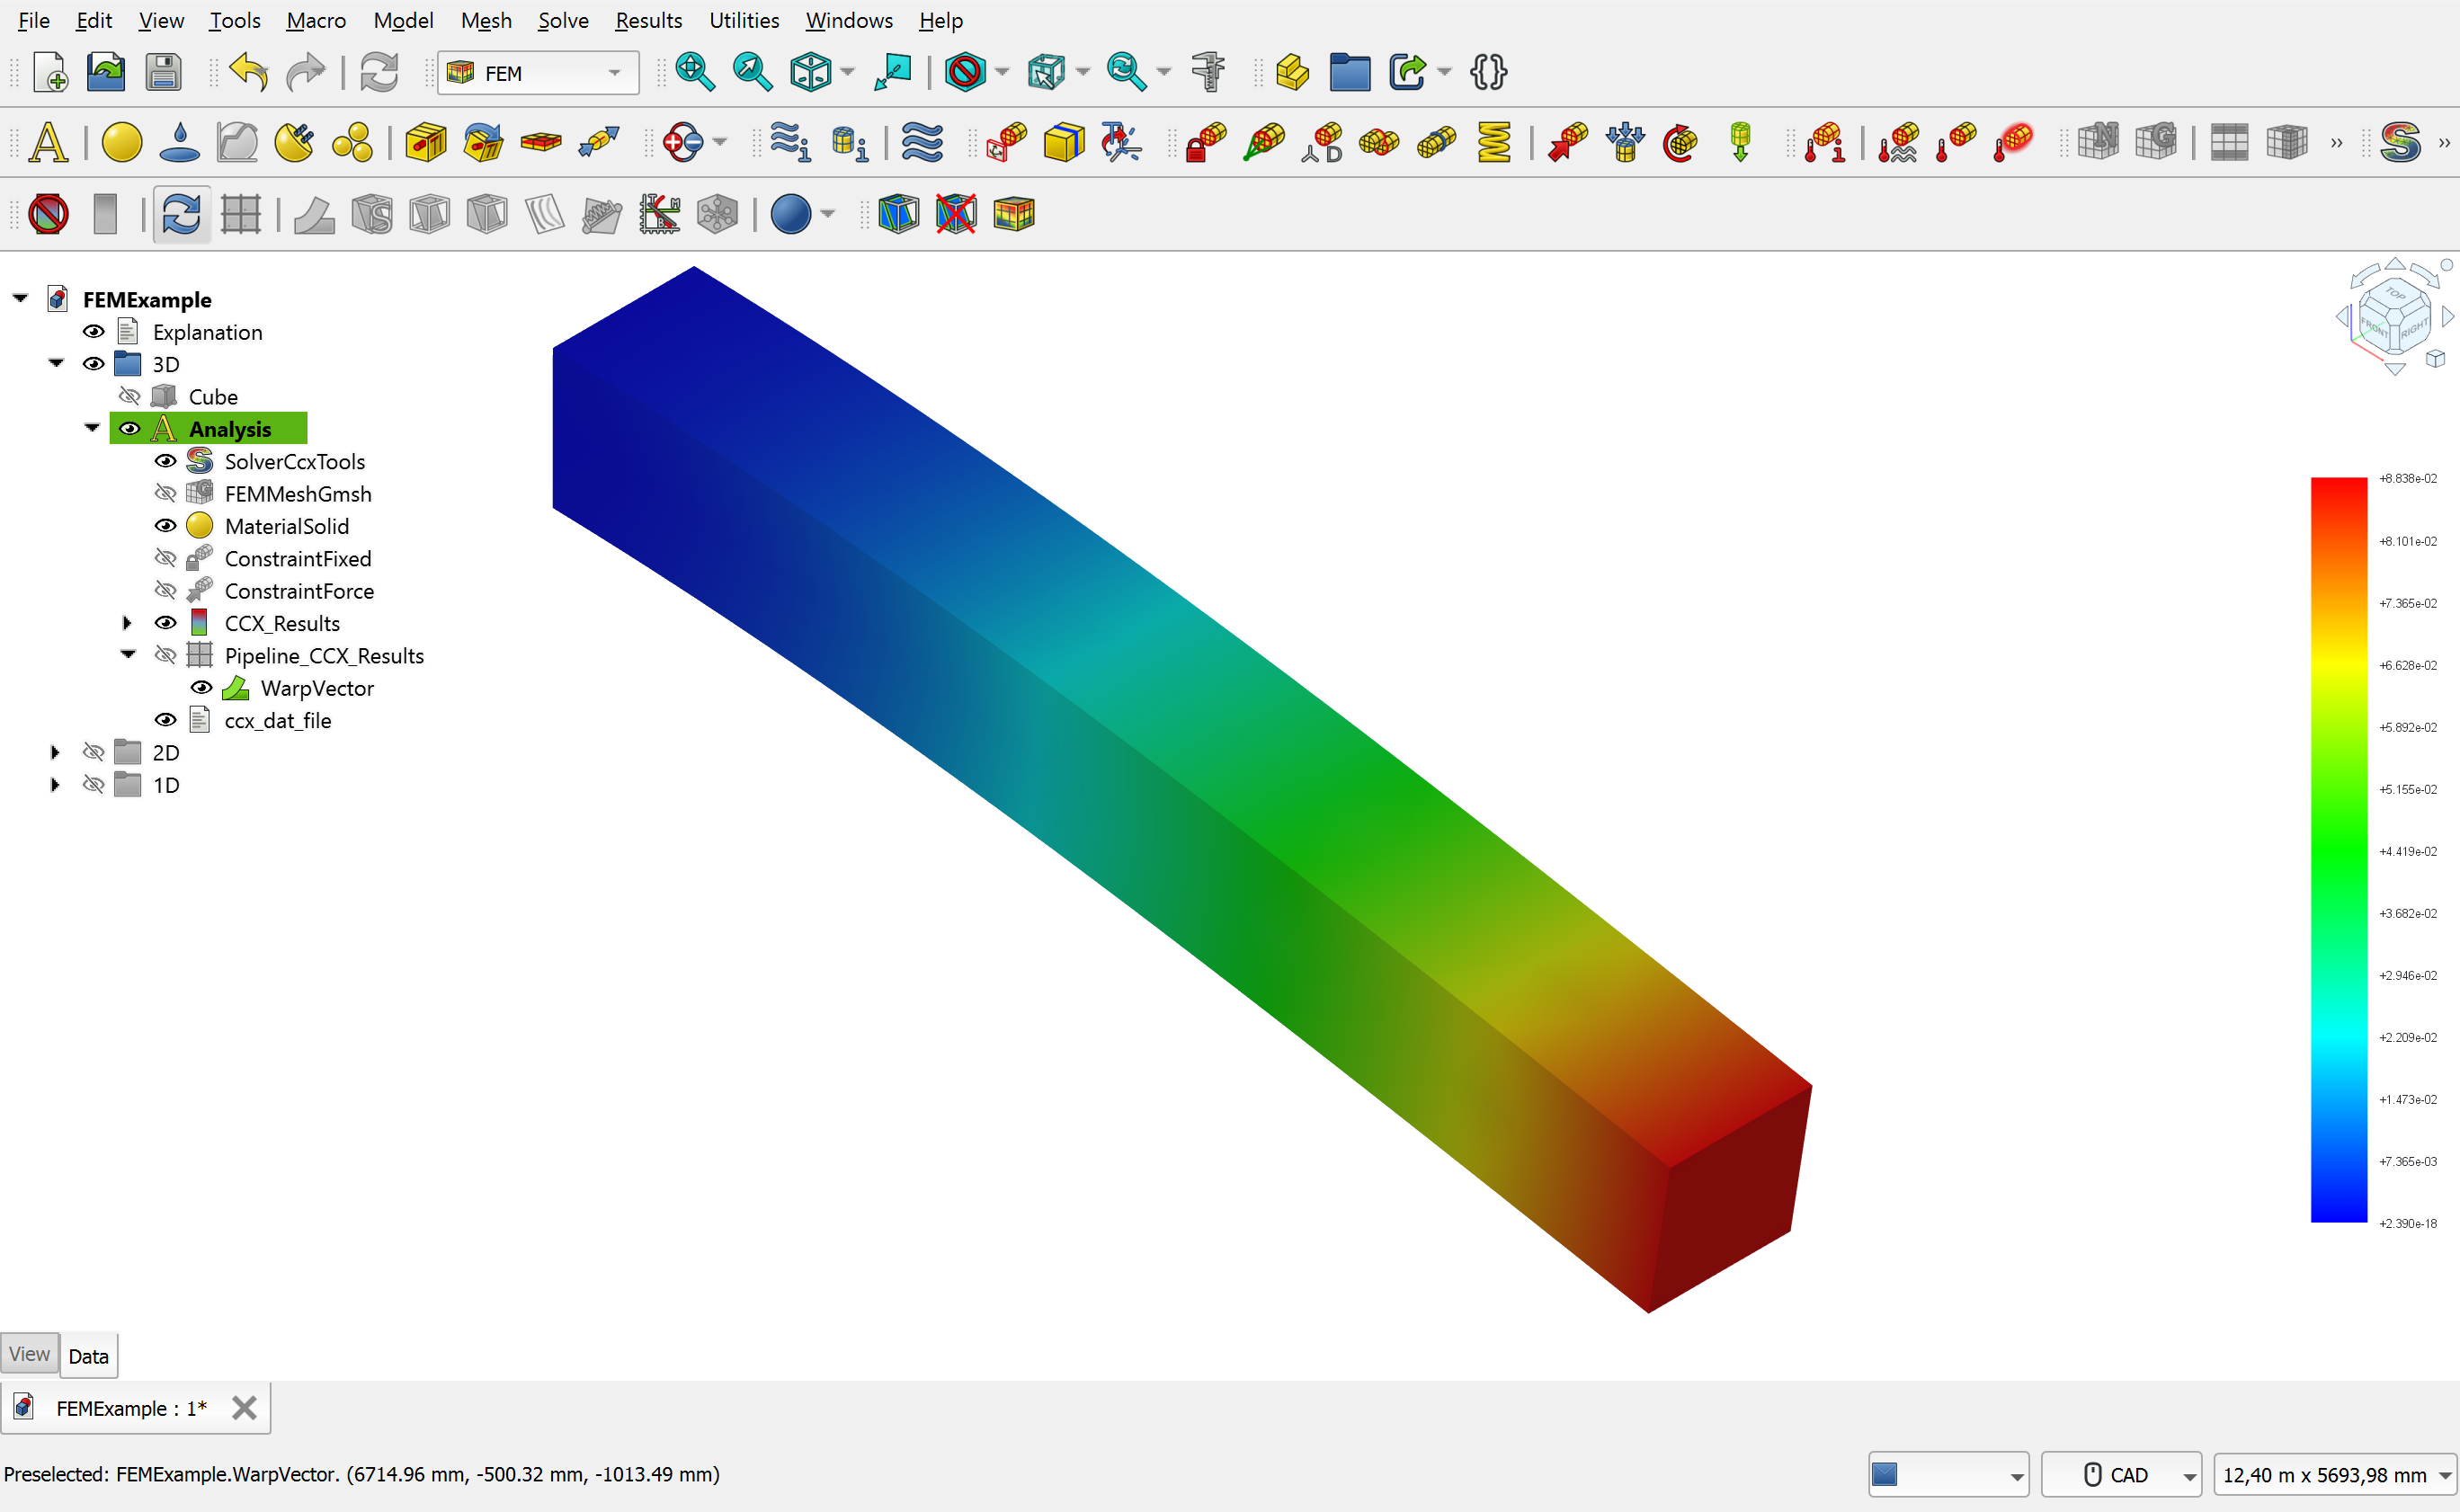
\includegraphics[width=0.8\textwidth]{img/cap8_planos.png}
	\caption{Plano técnico generado con el módulo TechDraw}
\end{figure}

Aprende a crear planos técnicos profesionales con
FreeCAD. Genera documentación técnica a partir de
modelos 3D usando el módulo TechDraw.

%% D. Búsqueda e Inserción de Activos Gráficos
%% Imagen insertada al inicio del capítulo

%% B. Actividades Teóricas
\section{Investigar y responder}
\faPencil

Investiga sobre planos técnicos en FreeCAD y responde:
\begin{enumerate}
	\item ¿Qué es un plano técnico y para qué sirve?
	\item ¿Cuáles son las vistas principales en un plano?
	\item ¿Cómo se generan vistas ortográficas desde un
	      modelo 3D?
	\item ¿Qué son las cotas de referencia y de cota?
	\item ¿Cómo se añaden anotaciones y símbolos a un plano?
	\item ¿Qué formatos de exportación soporta TechDraw?
	\item ¿Cómo se personalizan los estilos de plano?
	\item ¿Qué normas técnicas se deben seguir en planos?
\end{enumerate}

%% C. Actividades Prácticas
\section{Resolver los siguientes problemas}
\faWrench

Problemas para aplicar conocimientos:
\begin{enumerate}
	\item Abre un modelo 3D existente en FreeCAD.
	\item Crea un nuevo plano usando el módulo TechDraw.
	\item Añade una vista frontal del modelo al plano.
	\item Añade vistas lateral y superior del modelo.
	\item Inserta cotas dimensionales en el plano.
	\item Añade una vista isométrica del modelo.
	\item Incluye leyenda y título en el plano.
	\item Exporta el plano a formato PDF.
	\item Personaliza los estilos de líneas y cotas.
	\item Crea un plano completo con todas las vistas
	      necesarias para fabricación.
\end{enumerate}
\chapter{Ensamblajes Básicos}

\begin{figure}[H]
	\centering
	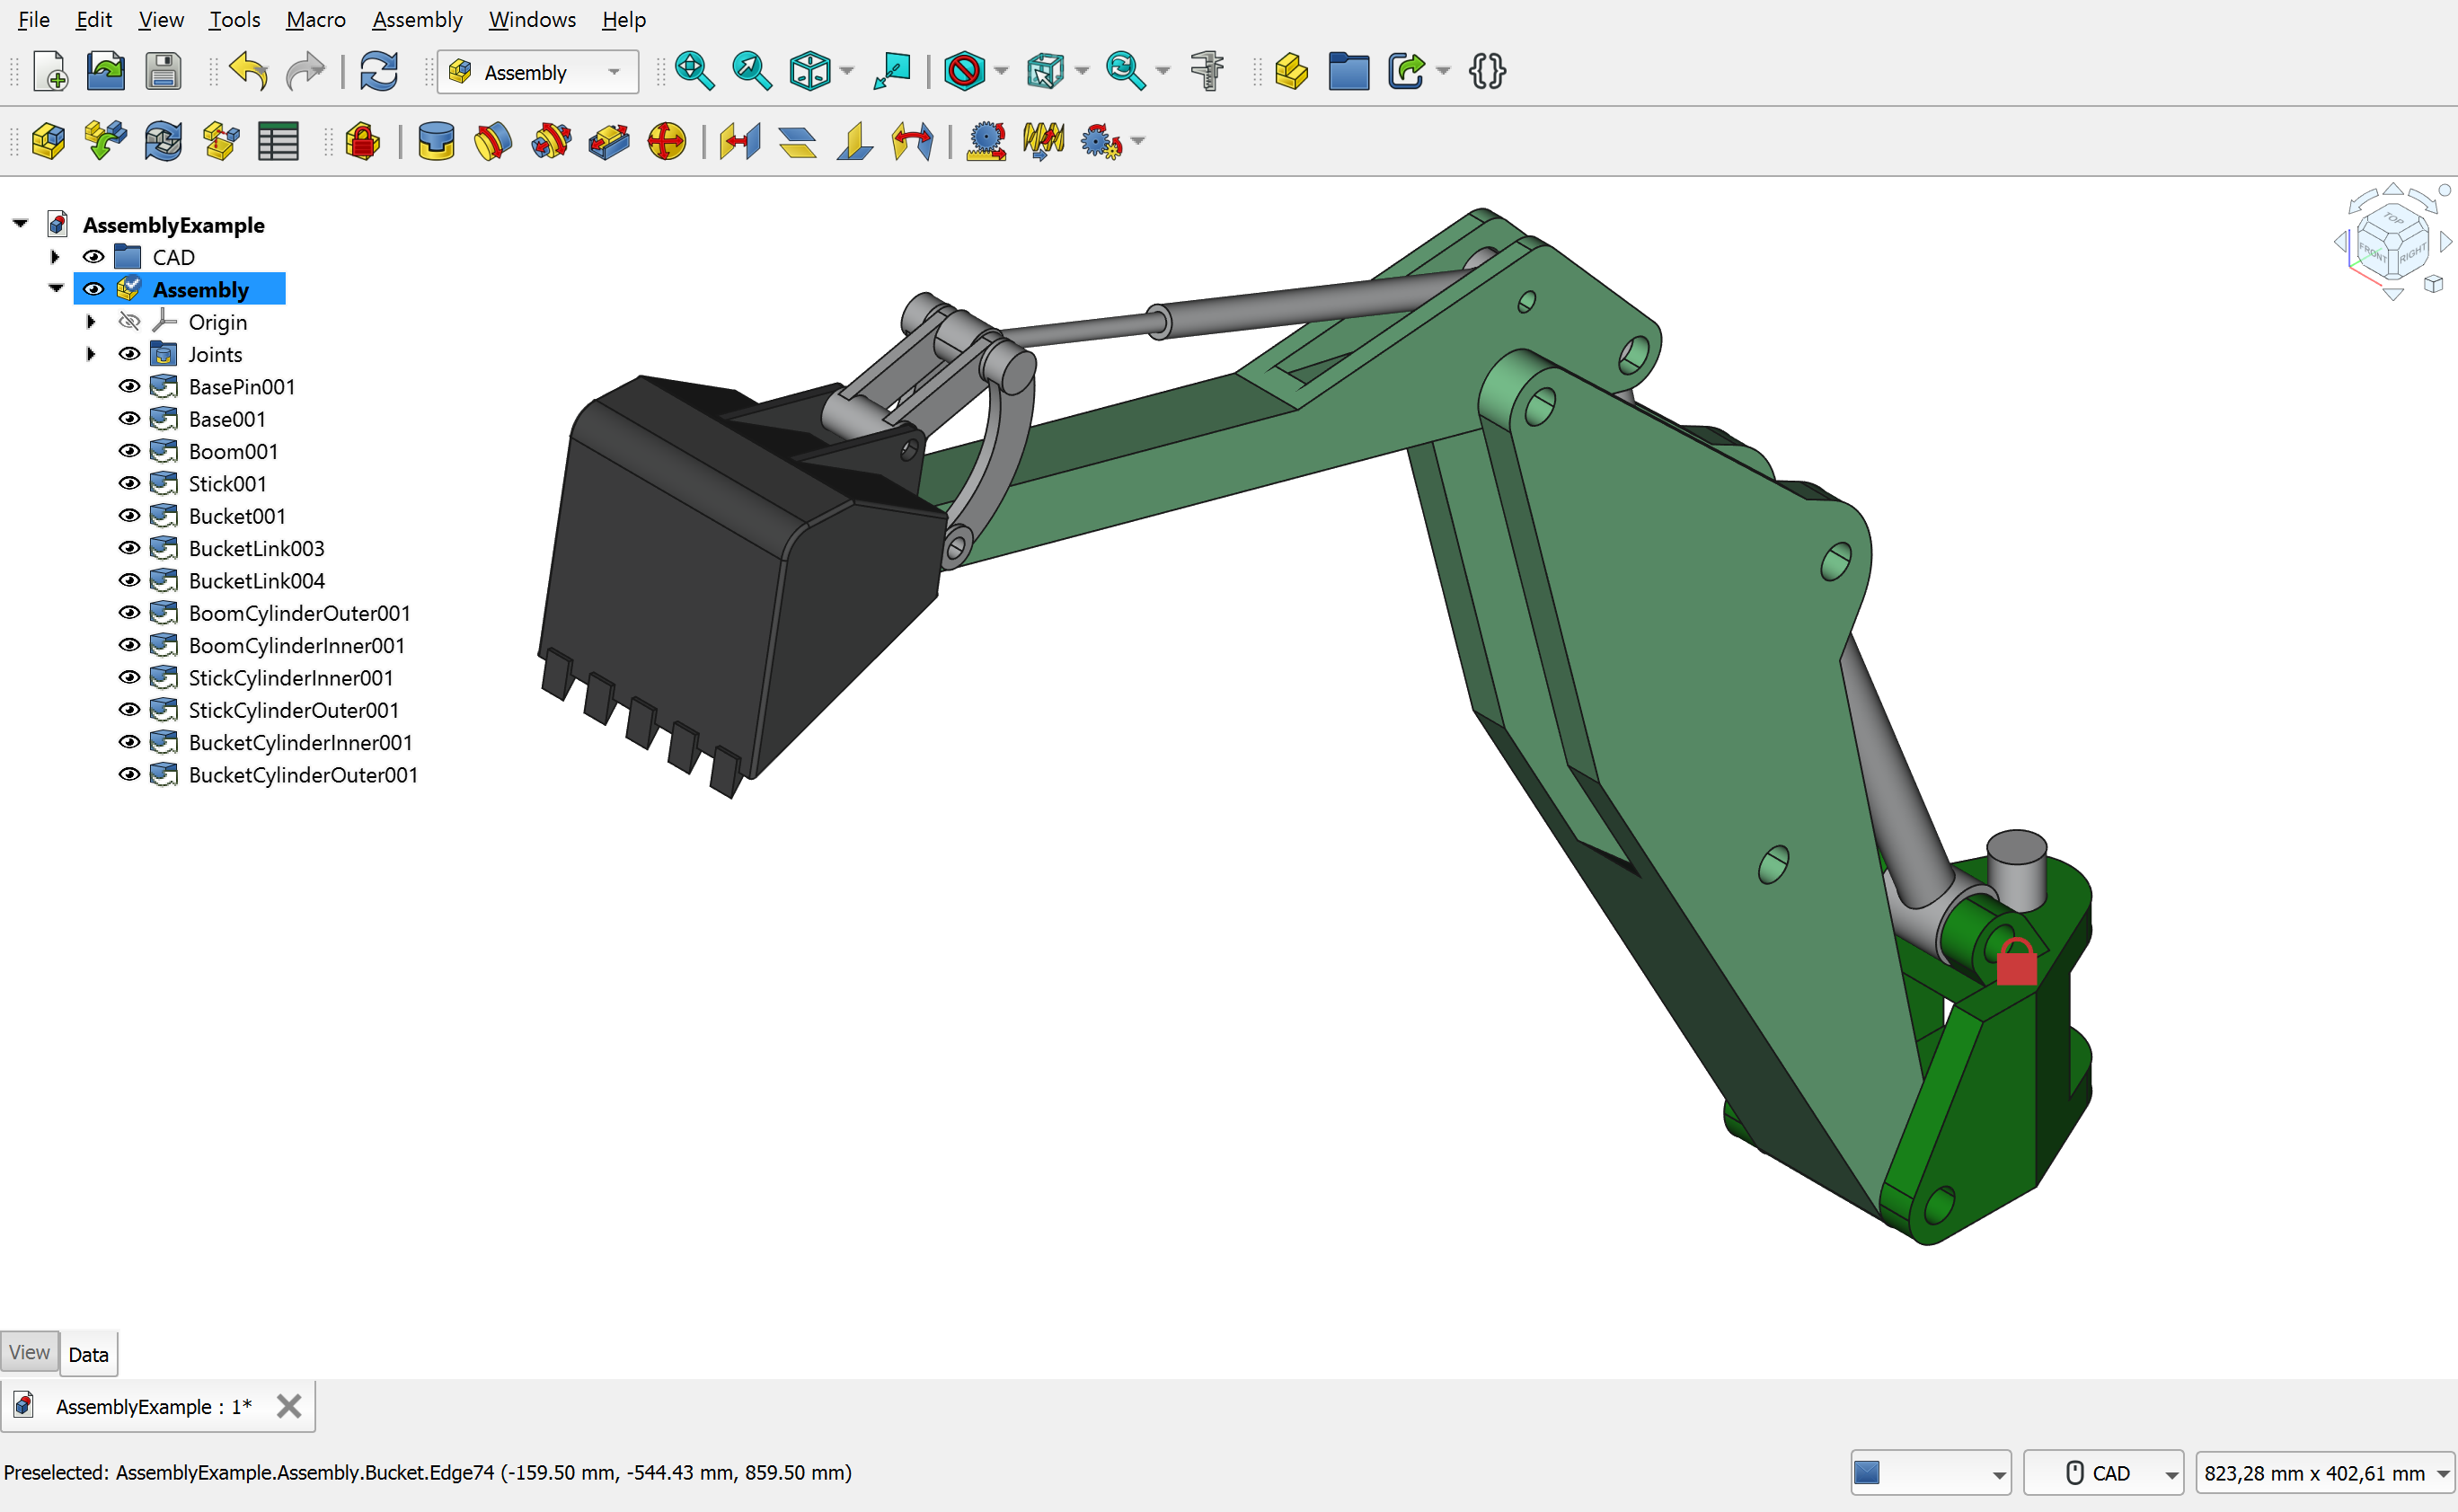
\includegraphics[width=0.8\textwidth]{img/cap9_ensamblajes.png}
	\caption{Ensamblaje de múltiples piezas en FreeCAD}
\end{figure}

Aprende a crear ensamblajes de múltiples piezas en
FreeCAD. Une componentes, define restricciones de
ensamblaje y crea mecanismos simples.

%% D. Búsqueda e Inserción de Activos Gráficos
%% Imagen insertada al inicio del capítulo

%% B. Actividades Teóricas
\section{Investigar y responder}
\faPencil

Investiga sobre ensamblajes en FreeCAD y responde:
\begin{enumerate}
	\item ¿Qué es un ensamblaje en diseño CAD?
	\item ¿Cómo se importan piezas externas en un archivo?
	\item ¿Qué tipos de restricciones de ensamblaje existen?
	\item ¿Cómo se definen relaciones de coincidencia?
	\item ¿Qué es la ``explosión'' de un ensamblaje?
	\item ¿Cómo se detectan interferencias entre piezas?
	\item ¿Qué plugins existen para ensamblajes en FreeCAD?
	\item ¿Cómo se crean listas de materiales (BOM)?
\end{enumerate}

%% C. Actividades Prácticas
\section{Resolver los siguientes problemas}
\faWrench

Problemas para aplicar conocimientos:
\begin{enumerate}
	\item Crea dos piezas simples separadas en archivos
	      diferentes.
	\item Importa ambas piezas en un nuevo archivo de
	      ensamblaje.
	\item Aplica una restricción de coincidencia entre
	      caras de las piezas.
	\item Añade una restricción de alineación entre
	      ejes de las piezas.
	\item Crea un ensamblaje de tres piezas con diferentes
	      tipos de restricciones.
	\item Practica la ``explosión'' del ensamblaje para
	      visualizar componentes.
	\item Detecta interferencias en un ensamblaje
	      mal restringido.
	\item Modifica la posición de una pieza después de
	      crear el ensamblaje.
	\item Crea un ensamblaje simple de un mecanismo
	      de biela-manivela.
	\item Exporta el ensamblaje a formato STEP para
	      intercambio con otros programas.
\end{enumerate}
\chapter{Diseño para Impresión 3D}

\begin{figure}[H]
	\centering
	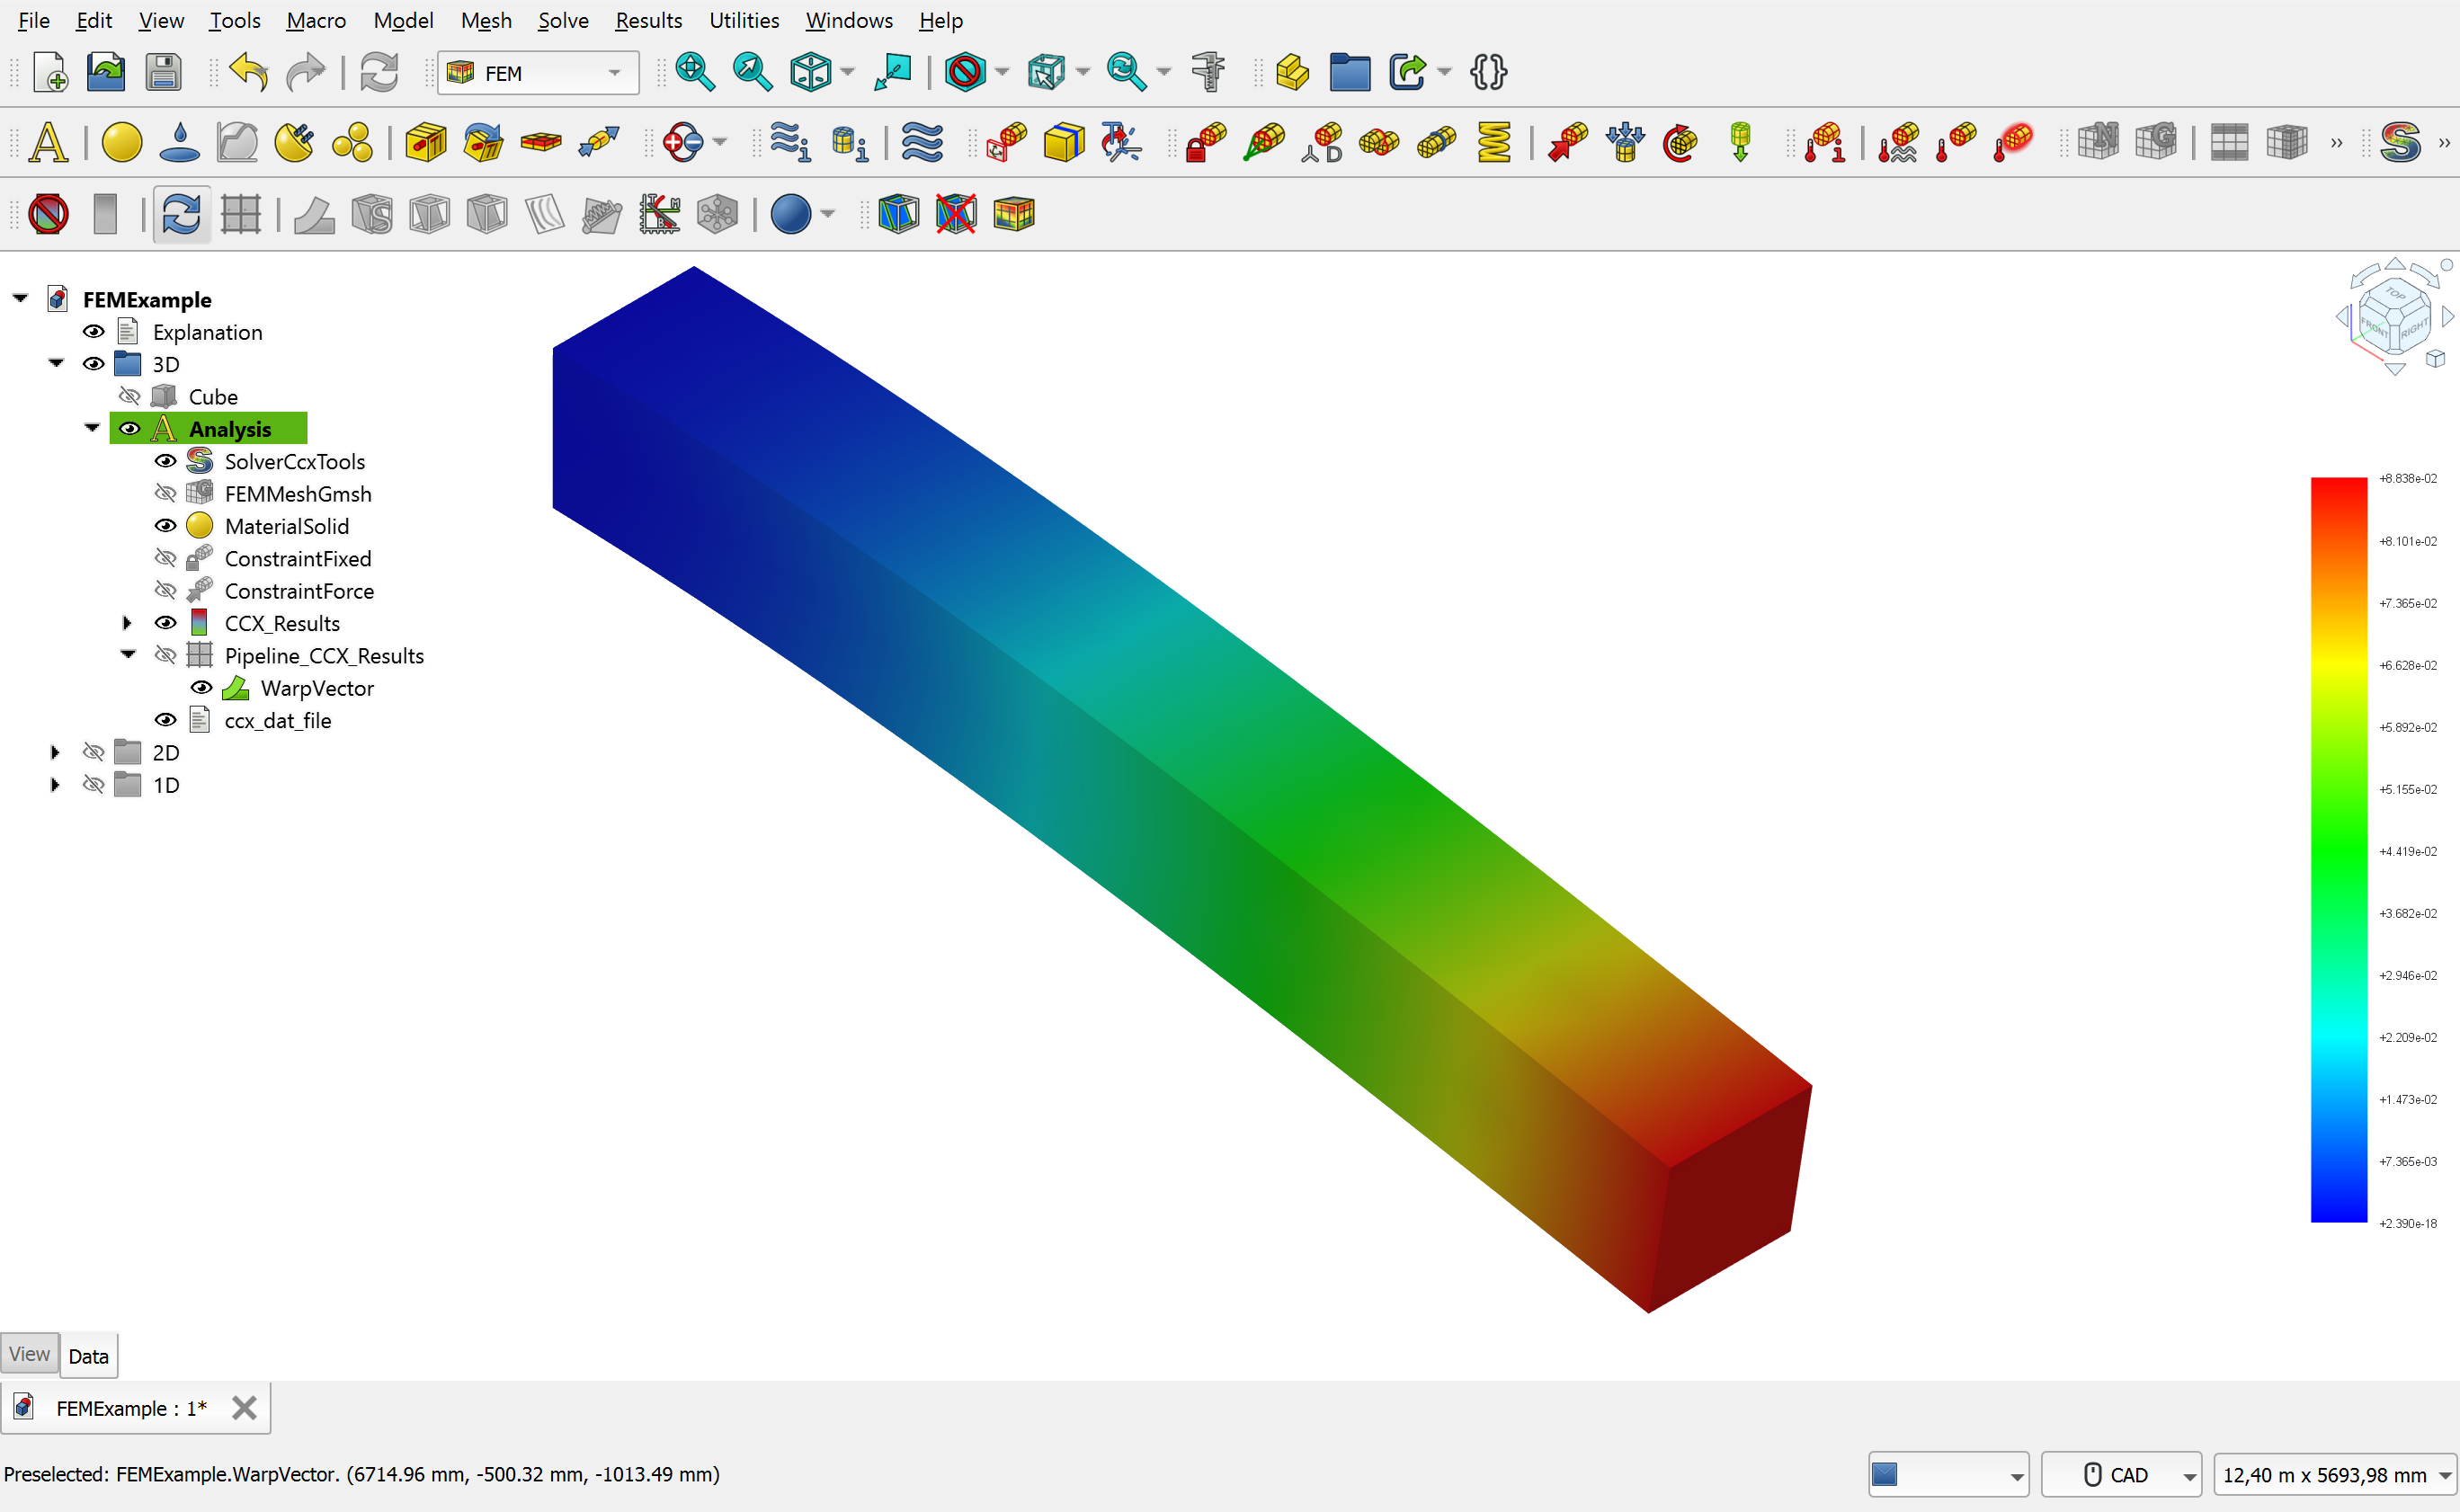
\includegraphics[width=0.8\textwidth]{img/cap10_impresion3d.png}
	\caption{Modelo optimizado para impresión 3D en FreeCAD}
\end{figure}

Aprende a diseñar modelos específicos para impresión 3D.
Optimiza tus diseños para fabricación aditiva y evita
errores comunes de impresión.

%% D. Búsqueda e Inserción de Activos Gráficos
%% Imagen insertada al inicio del capítulo

%% B. Actividades Teóricas
\section{Investigar y responder}
\faPencil

Investiga sobre diseño para impresión 3D y responde:
\begin{enumerate}
	\item ¿Qué es la fabricación aditiva (impresión 3D)?
	\item ¿Qué limitaciones tienen las impresoras 3D?
	\item ¿Cómo se exporta un modelo a formato STL?
	\item ¿Qué es el ``manifold'' y por qué es importante?
	\item ¿Cómo se verifican errores en mallas 3D?
	\item ¿Qué diseños son difíciles de imprimir en 3D?
	\item ¿Cómo se optimizan modelos para reducir tiempo
	      de impresión?
	\item ¿Qué formatos son recomendables para impresión 3D?
\end{enumerate}

%% C. Actividades Prácticas
\section{Resolver los siguientes problemas}
\faWrench

Problemas para aplicar conocimientos:
\begin{enumerate}
	\item Diseña un soporte para teléfono celular optimizado
	      para impresión 3D.
	\item Exporta tu modelo a formato STL y verifica su
	      integridad.
	\item Diseña una pieza con soportes internos para
	      mejorar resistencia.
	\item Crea un modelo con paredes de espesor mínimo
	      recomendado.
	\item Diseña una pieza que evite voladizos pronunciados.
	\item Optimiza un modelo existente reduciendo cantidad
	      de material.
	\item Verifica que tu modelo no tenga huecos internos
	      o errores de malla.
	\item Diseña un encaje tipo ``snap-fit'' para ensamblaje
	      sin pegamento.
	\item Practica el diseño de piezas con texturas o
	      patrones para impresión.
	\item Prepara un modelo para impresión incluyendo
	      orientación y soportes.
\end{enumerate}
\chapter{Proyecto Integrador: Componente Mecánico}

\begin{figure}[H]
	\centering
	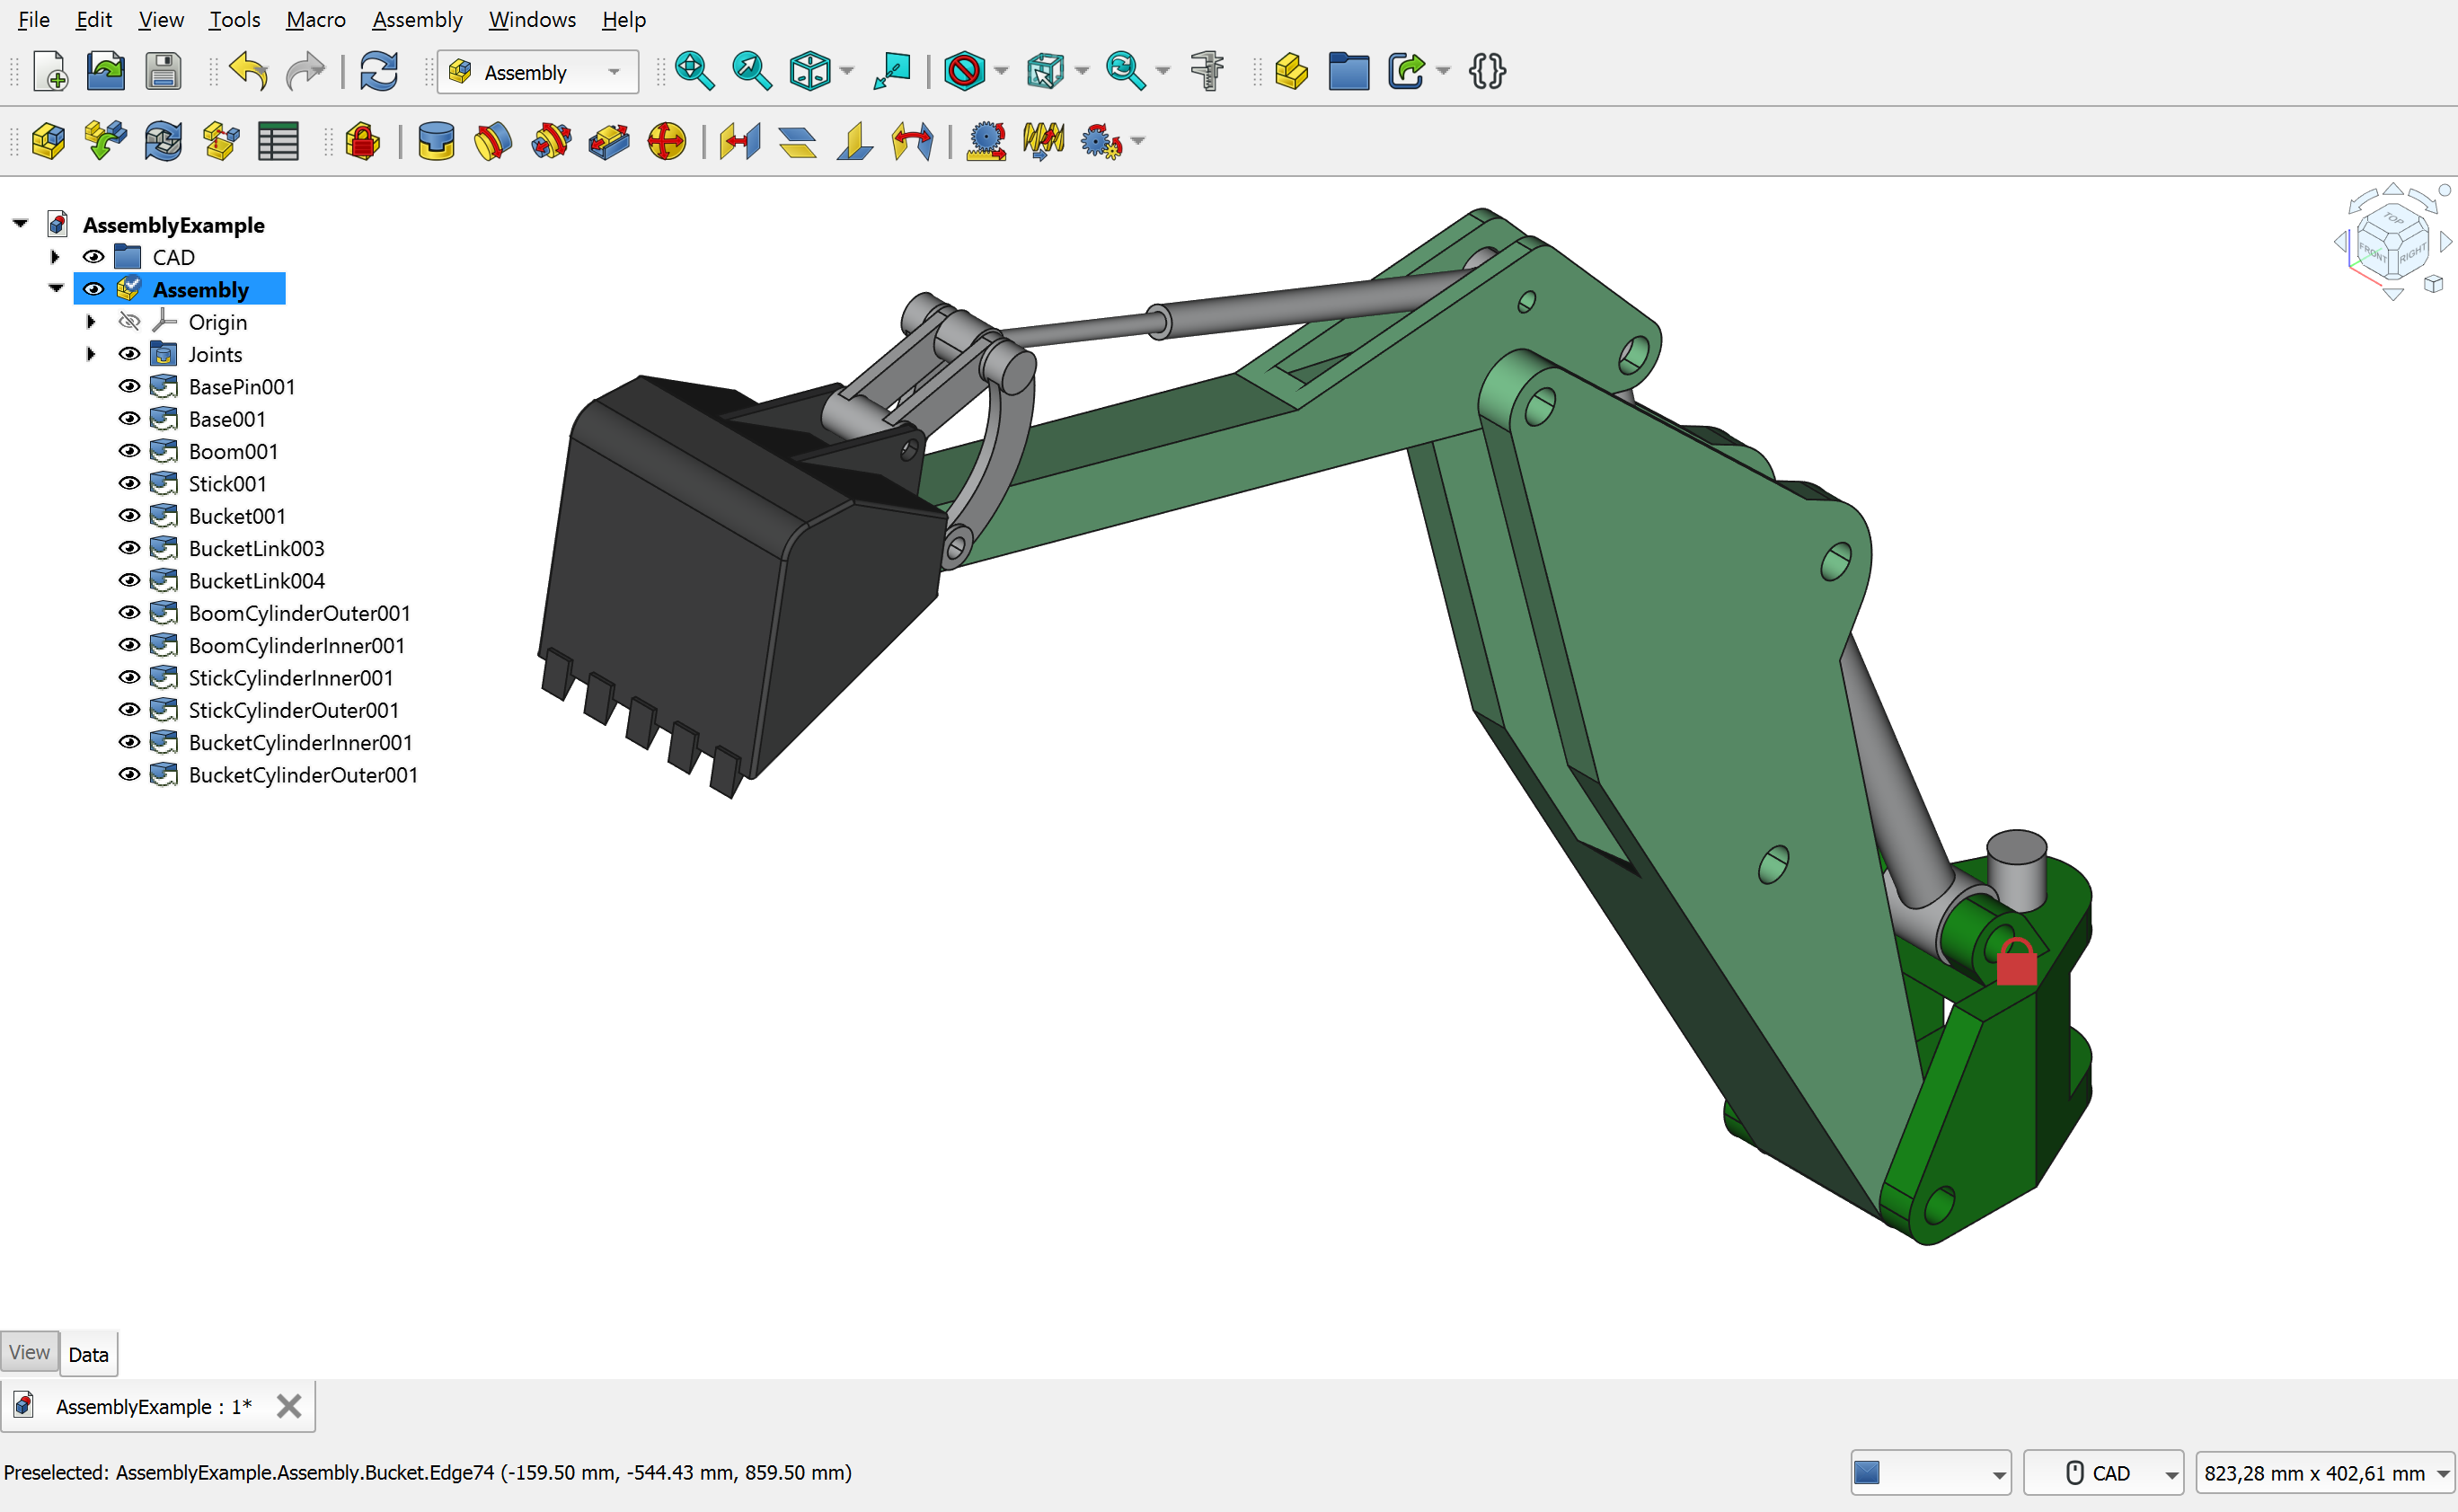
\includegraphics[width=0.8\textwidth]{img/cap11_proyecto.png}
	\caption{Componente mecánico completo diseñado en FreeCAD}
\end{figure}

Proyecto final que integra todos los conocimientos
aprendidos. Diseña un componente mecánico completo
siguiendo estándares de la industria argentina.

%% D. Búsqueda e Inserción de Activos Gráficos
%% Imagen insertada al inicio del capítulo

Proyecto: Soporte para maquinaria agrícola
\begin{itemize}
	\item Sector: Industria agropecuaria argentina
	\item Normas: IRAM y estándares industriales
	\item Requisitos: Resistencia, facilidad de fabricación
\end{itemize}

%% B. Actividades Teóricas
\section{Investigar y responder}
\faPencil

Investiga sobre el proyecto y responde:
\begin{enumerate}
	\item ¿Qué es un soporte mecánico y qué funciones cumple?
	\item ¿Qué materiales se usan comúnmente en soportes
	      agrícolas?
	\item ¿Qué normas argentinas aplican a componentes
	      mecánicos?
	\item ¿Cómo se determinan las cargas que soportará
	      el componente?
	\item ¿Qué procesos de fabricación son comunes en
	      Argentina?
	\item ¿Cómo se asegura la calidad de un componente
	      mecánico?
	\item ¿Qué consideraciones de seguridad deben tenerse?
	\item ¿Cómo se documenta técnicamente un componente
	      industrial?
\end{enumerate}

%% C. Actividades Prácticas
\section{Resolver los siguientes problemas}
\faWrench

Problemas para aplicar conocimientos:
\begin{enumerate}
	\item Diseña el boceto principal del soporte con
	      dimensiones aproximadas.
	\item Aplica restricciones geométricas y dimensionales
	      al boceto.
	\item Crea el sólido principal usando operación de
	      extrusión.
	\item Añade agujeros para tornillería estándar.
	\item Aplica biselados y chaflanados según requerimientos.
	\item Diseña los componentes de sujeción complementarios.
	\item Crea un ensamblaje completo del soporte con
	      tornillería.
	\item Genera planos técnicos con todas las vistas
	      necesarias.
	\item Exporta modelos a STL para posible impresión
	      3D.
	\item Documenta el proyecto completo con especificaciones
	      técnicas y conclusiones.
\end{enumerate}

\section{Evaluación del Proyecto}
\begin{itemize}
	\item Complejidad geométrica: 25 puntos
	\item Uso de restricciones: 20 puntos
	\item Operaciones de modelado: 25 puntos
	\item Planos técnicos: 20 puntos
	\item Documentación: 10 puntos
\end{itemize}

Total: 100 puntos

\bibliographystyle{plain}
\bibliography{bib/referencias}

\end{document}

